\documentclass[11pt, a4paper]{article}

\usepackage{varioref}
\usepackage{hyperref}
\usepackage{cleveref}

\usepackage{listings}
\usepackage{subfigure}
\usepackage{graphicx}
\usepackage{titling}
% \usepackage[margin=1.8cm, includefoot]{geometry}

\usepackage{parskip}
\setlength{\parindent}{0cm}

\usepackage{titlesec}
\usepackage{pdfpages}

\usepackage{framed}


% Select what to do with todonotes: 
% \usepackage[disable]{todonotes} % notes not showed
\usepackage[draft]{todonotes}   % notes showed

\newlength\longest
\interfootnotelinepenalty=10000
\titlespacing\section{0pt}{6pt plus 2pt minus 2pt}{0pt plus 0pt minus 2pt}
\titlespacing\subsection{0pt}{4pt plus 2pt minus 2pt}{0pt plus 0pt minus 2pt}
\newcommand{\subtitle}[1]{
  \posttitle{
    \par\end{center}
    \begin{center}\large#1\end{center}
    \vskip0.5em}
}

\setlength{\droptitle}{-4em}

\newcommand{\cmd}[1]{{\tt #1}}

\begin{document}

\title{Deeva}
\subtitle{A Java Debugger Suitable for Teaching}
\author{Kritaphat Sonsri-in, Xueqi Chen, Hector Dearman, \\Alina Draganescu, Felix de Souza}

\maketitle
\thispagestyle{empty} % No page numbers on first page.

% Report editing rules:
% Each sentence on a new line.
% Only edit one section before committing.
% Push after every commit.
% ONLY EDIT ONE SECTION BEFORE COMMITTING.



% Three main goals:
% 1. Fill a tool hole for first year Java course
% 2. Foster a strong mental model of imperative programming
% 3. Introduction to debugging

% Introduction 
%   Set the scene (‘motivation’) 
%   State the problem you are trying to solve (‘objective(s)’) 
%   Summarise what you achieved (‘contributions’) 
% Design & implementation 
%   Detail your design (why did you do it this way?) 
%   Summarise key implementation details (how did you do it? what tools did you use?) 
% Evaluation 
%   Summarise testing procedures (+ relevant testing results) 
%   Evaluate your deliverables, e.g. in terms of performance, usability, usefulness… 
%   (how successful was the project?) 
% Conclusion and future extensions 
%   Say what you’ve concluded from doing the work and how you’d build on it 
% Project management 
%   Planning, group organisation, breakdown + task allocation etc

\section*{Executive Summary}
\addcontentsline{toc}{section}{Executive Summary}

Deeva is a simple Java debugger for teaching which allows graphical introspection of a running program.

In the first year introductory Java course many students are encountering imperative programming for the first time so there is a strong desire to minimise `magic' particularly in the form of complex IDEs which `make it work'.
Unfortunately this attempt is hamstrung by the absence of a good Java debugger decoupled from an IDE.
Without a good strategy to fix broken programs students quickly reinvent bad habits ranging from the awful, shotgun debugging, to the merely poor, print statements.

What we want is debugger, invokable from the command line, simple enough that students who have never seen a debugger before can taught to use it in only a few minutes but powerful enough to make tracking down a bug easy. 
Deeva fills this hole in the Java ecosystem and Lab infrastructure.

Deeva was designed with an additional goal in mind.
At Imperial (as most places) students are taught imperative programming with diagrams, the lecturer draws a stack and a heap and shows how moving through the code effect the stack and the heap.
By using a novel user interface which resembles these diagrams we make debugging more intuitive, allow lectures to easily construct and step through these diagrams live on arbitrary code without fear of mistake and, for the first time, allow students to see how code they write is run on their own time without outside help.
This way Deeva becomes a tool for both teaching and learning.

All to many programmers, experts and beginners, never really learn to use or desire the powerful tools which already exist to introspect and modify running programs preferring instead to grovel though the source code with \cmd{printf}.
For students Deeva provides excellent introduction to these tools while also filling a vital gap in Lab infrastructure and providing a useful tool for lecturers teaching imperative programming.


% What is a debugger?
% ``Bugs'' are a type of software defect typically introduced though a mismatch between the programmers mental model of the system and the system itself.
% A ``debugger'' then is a program that allows programmers to inspect and manipulate the state and flow of a running system so they can understand the mismatch and hence fix the defect.

% Specifically students are encouraged to use a text editor and invoke the Java compiler and virtual machine directly in order develop a deeper and more transferable understanding of programming.
% 
% first to help foster a strong mental model of imperative programming and secondly to introduce students to powerful introspection of software systems.

%the Imperial Computing department attaches great importance to practical programming ability much of students first year is spent learning several programming languages and completing many Labs, small programming tasks. 
%The practical teaching of programming on the first year follows this progression: Functional programing, Imperative programing, Object Orientation and finally Systems programming.
%Historically the department has taught Functional programming using Haskell, OO programming using Java and Systems programming using C but for Imperative programing a few different approaches have been tried.

\clearpage
\tableofcontents
\clearpage

\section{Motivation}
\subsection{``Introduction to Imperative Programming" at Imperial}
Around half of first year undergraduate computing students at Imperial have no previous imperative programming experience\cite{projectproposal} so the course ``Introduction to Imperative Programming" run in the first term after directly after ``Introduction to Functional Programming" forms a cornerstone of the practical education students receive giving them skills they will need almost every other course.

The course focuses on the basics: control flow, functions and the write, compile, run cycle.
To make teaching more effective it is desirable to avoid introducing unnecessary complexity like Object Orientation, memory management or complex IDEs all of which are left to later courses.
For example although the class is now taught in Java () it has previously been taught in Kenya\footnote{} a language which acts as an imperative stepping stone to Java by allowing functions to exist outside of objects.

In particular department does not want students to end up relying on the large complex IDE like Eclipse or IntelliJ to `magically' run the code without understanding what it does.
So recently \todo{fact check} \footnote{For the last two years.} students have been encouraged to avoid IDEs and instead use a text editor (like \cmd{vim}, \cmd{emacs} or \cmd{gedit}) and invoke the Java compiler (\cmd{javac}) and virtual machine (\cmd{java}) directly.
Unfortunately there is downside to this approach, most Java debuggers are integrated into IDEs and those which are not are often of poor quality, this coupled with the relatively complex UI of debuggers in general (see our analysis below) means that there is no good option for instructors to suggest to students.
Students quickly encounter bugs in their programs and (necessarily) without a strong understanding of the language or a taught strategy to deal with bugs they are reduced to reinventing well known bad habits including \todo{list of bad habits}.

To combat this problem Dr. Tristan Allwood proposed\cite{projectproposal} this third year group project to build a tool to fill this gap.
A debugger which was: independent from an IDE, simple enough to be 	used by beginners but powerful enough to be useful.

The project also had another goal which was to be a tool for teaching.
In ``Introduction to Imperative Programming" teaches fundamentals including control flow and the effect of assignment and function calls, return statements, etc
\footnote{A strong mental model of programming fundamentals very important, for example when learning to program an early, consistent grasp of assignment is predictive of eventual achievement\cite{saeed09}.}.
As in many courses this is done diagrammatically, by showing how each line of code in a program effects the stack and heap.

\begin{figure}[h!]
\centering
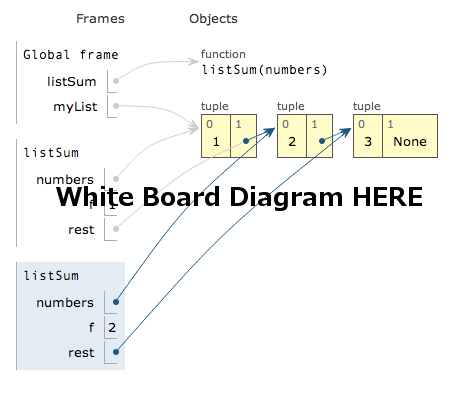
\includegraphics[width=100mm]{whiteboard.png}
\caption{Example diagram of Stack and Heap}
\end{figure}

However this approach is not ideal.
It is time consuming and error prone to update the diagram and worse it requires an oracle, the instructor, to act as mechanical interpreter of the rules.
Students have no way see such a visualisation on arbitrary code they write, no easy way to see why code they write does not have the effect they expect without ad-hoc experimentation: modifying the source code and hoping it exposes the original problem.

All of these problems are the kind that computers are very good at and indeed tools like \cmd{Python Tutor}\cite{pythontutor} can take a code snippet and produce visualisation of the execution trace. 

\begin{figure}[h!]
\centering
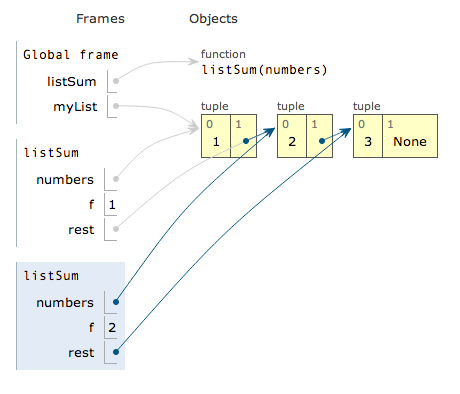
\includegraphics[width=100mm]{PythonTutorStackHeap.png}
\caption{Python Tutor Stack and Heap Diagram}
\end{figure}

By replacing the unintuitive tabular representation of the stack and heap found in almost every debugger with a user interface based these diagrams we hope to make Deeva a useful tool for teaching.
Allowing instructors to quickly create traces for programs in real time without the possibility of mistake.
Even more importantly it lets Deeva become a tool for learning allowing students to explore the unfamiliar model of imperative programming without expert oversight.


Finally despite the existence of powerful tools to introspect running programs many programmers continue to debug programs using print statements.
Since

\todo{something}


\subsection{Alternatives}
As part of our requirement analysis stage, we looked into detail of various existed debuggers to compare their pros and cons, and their suitability for first year students.

\subsubsection{jdb}
\begin{figure}[h!]
\centering
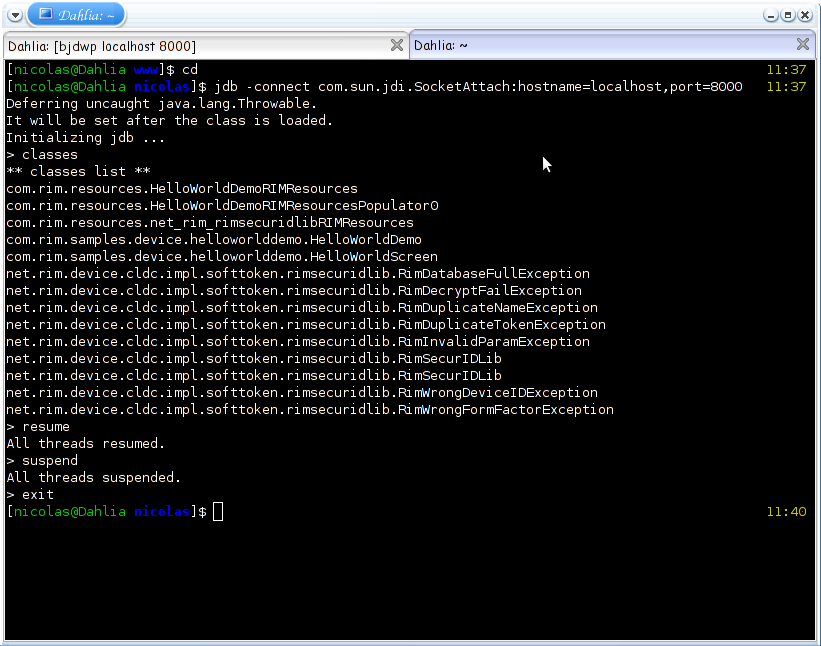
\includegraphics[width=100mm]{jdb.png}
\end{figure}

The Java Debugger, jdb, is a simple command line debugger that provides inspection and debugging for Java classes.
It provides most of the basic functionalities of a debugger eg. setting breakpoint(s), stepping through the next line, and diagnosing the cause of the exception.
However, since it is a command line debugger, it provides a poor graphic user interface.
Hence, it is not quite intuitive to use.
\subsubsection{JSwat}
\begin{figure}[h!]
\centering
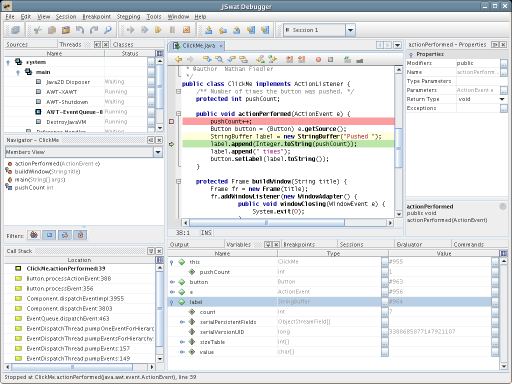
\includegraphics[width=100mm]{jswat.png}
\end{figure}

JSwat is a graphical Java debugger which provides basic functionality like: setting breakpoints, thread and stack display, variable monitoring and method invocation.
The feature it has which is lacking in some other debuggers is it allows users to trace through a linked list nicely by just clicking on a certain button repeatedly.
A benefit of it is its small size, in terms of the disc usage.
However, its unattractive interface with varies of features might still be a overwhelm for first year students.
\subsubsection{Eclipse Debugger}
\begin{figure}[h!]
\centering
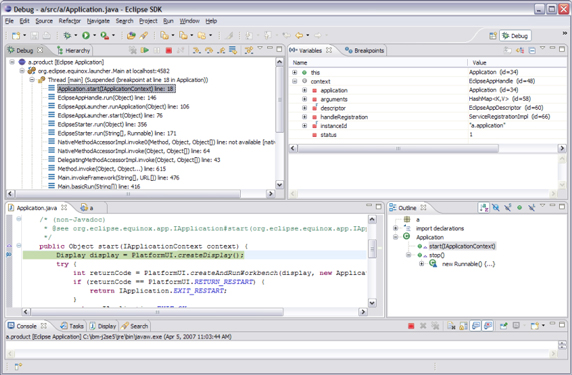
\includegraphics[width=100mm]{eclipse.jpg}
\end{figure}

Eclipse allows starting a Java program in Debug mode which provides a control of the execution process of the program and allows investigation of the state of the variables.
In addition, it provides a lot more functionalities than jdb such as setting a conditional breakpoints, variables modification, and having an user friendly graphic user interface.
Nevertheless, being an integrated IDE debugger and having a lot of unused features for beginner, it might overwhelm first year students.
\subsubsection{IntelliJ Debugger}
\begin{figure}[h!]
\centering
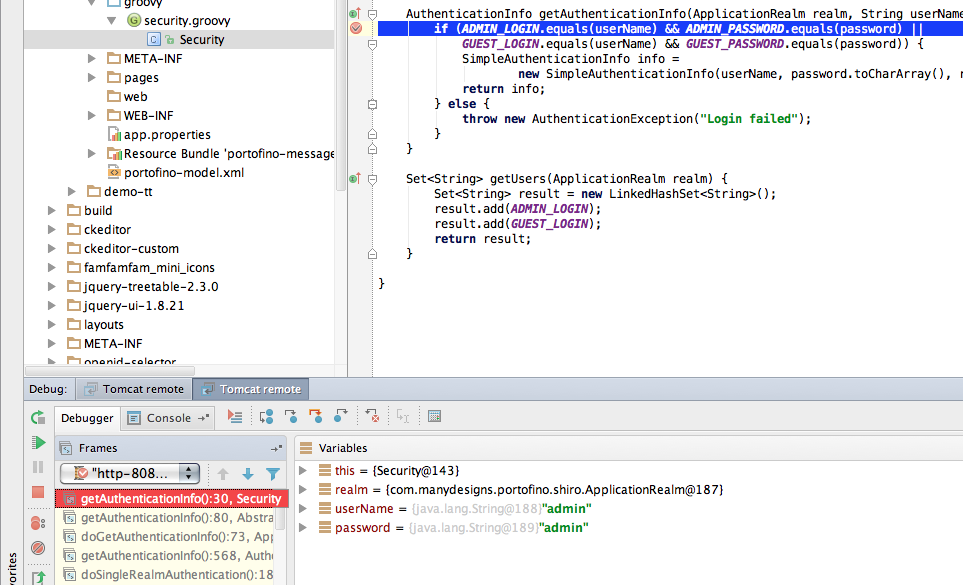
\includegraphics[width=100mm]{intellij.png}
\end{figure}

Similar to Eclipse Debugger, IntelliJ Debugger is also an integrated IDE debugger which provides fast and powerful functionalities.
Even though it also provides nice feature that allow object(s) inspection easier, its overwhelming functionalities may cumbersome first year students.
\subsubsection{Python Tutor}
\begin{figure}[h!]
\centering
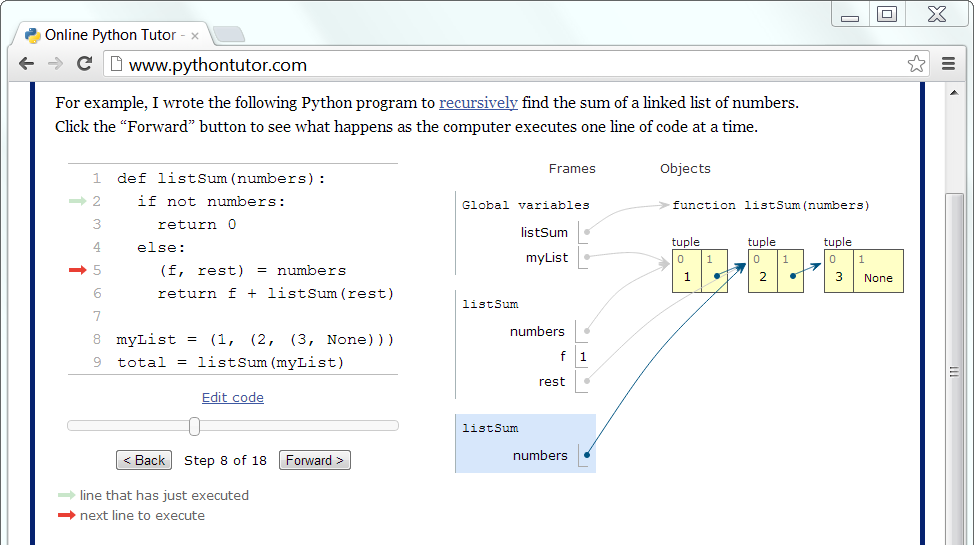
\includegraphics[width=100mm]{pythontutor.png}
\end{figure}

Python Tutor is a debugger that provides users with a visualisation of the program.
A user can write a Python program in the web browser and visualise what happens as the computer executes each line of the code.
It is also capable of going backwards, the key functionality that distinguishes it from other debuggers.
This would be the optimal choice for our first year students except that it works for Python not Java.
However this would be what we are aiming to design.

\section{Objectives} 

To produce a Java debugger that was:

\begin{description}
\item[Independent] \hfill \\
\item[Powerful] \hfill \\
\item[Simple] \hfill \\
\end{description}

At the start of the project we produced a initial plan (for the full plan please see ~\cref{sec:initialplan}) where we broke these high level objectives down into a minimal set of concrete goals which we then had signed off by Dr. Allwood.

\begin{itemize}
\item Must run in the Labs
\item Start from the command line
\item Supporting all the command line switches (-ea etc)
\item Taking command line arguments (from the gui)
\item Users must be able to see stdin, stdout, stderr
\item Users must be able to see the source code
\item Users must be able to inspect the current state of the program somehow
\item Run/Pause/Step into/Step Over
\item Multiple Files
\item Breakpoints
\item Supports Java static methods, Objects, Arrays, Control flows, Generics, Enumerations
\item Minimal Documentation (--help, README, small user guide, etc)
\end{itemize}

Similarly we produced a prioritised list of extensions:

\begin{enumerate}
\item Lecture Mode
\item Display of state is graphical
\item Pictures of previous state and current state for comparison
\item Conditional breakpoints
\item Watch points
\item Multi-platform (OSX, Linux, Windows)
\item Maximal Documentation
\item Support all of Java (Threads etc)
\end{enumerate}


\section{Deeva}
\todo{Big section where we describe each feature of Deeva in detail.}


\section{Design}
\subsection{Deciding on a Web Frontend}
During the meeting that we arranged with Tristan, we talked through what we had understood from the specification for the project.
We also asked him to go through his expectations in details so that we could get a full understanding on the project.
Hence a sketch of the original design was generated based on the requirements. 
\begin{figure}[h!]
\centering
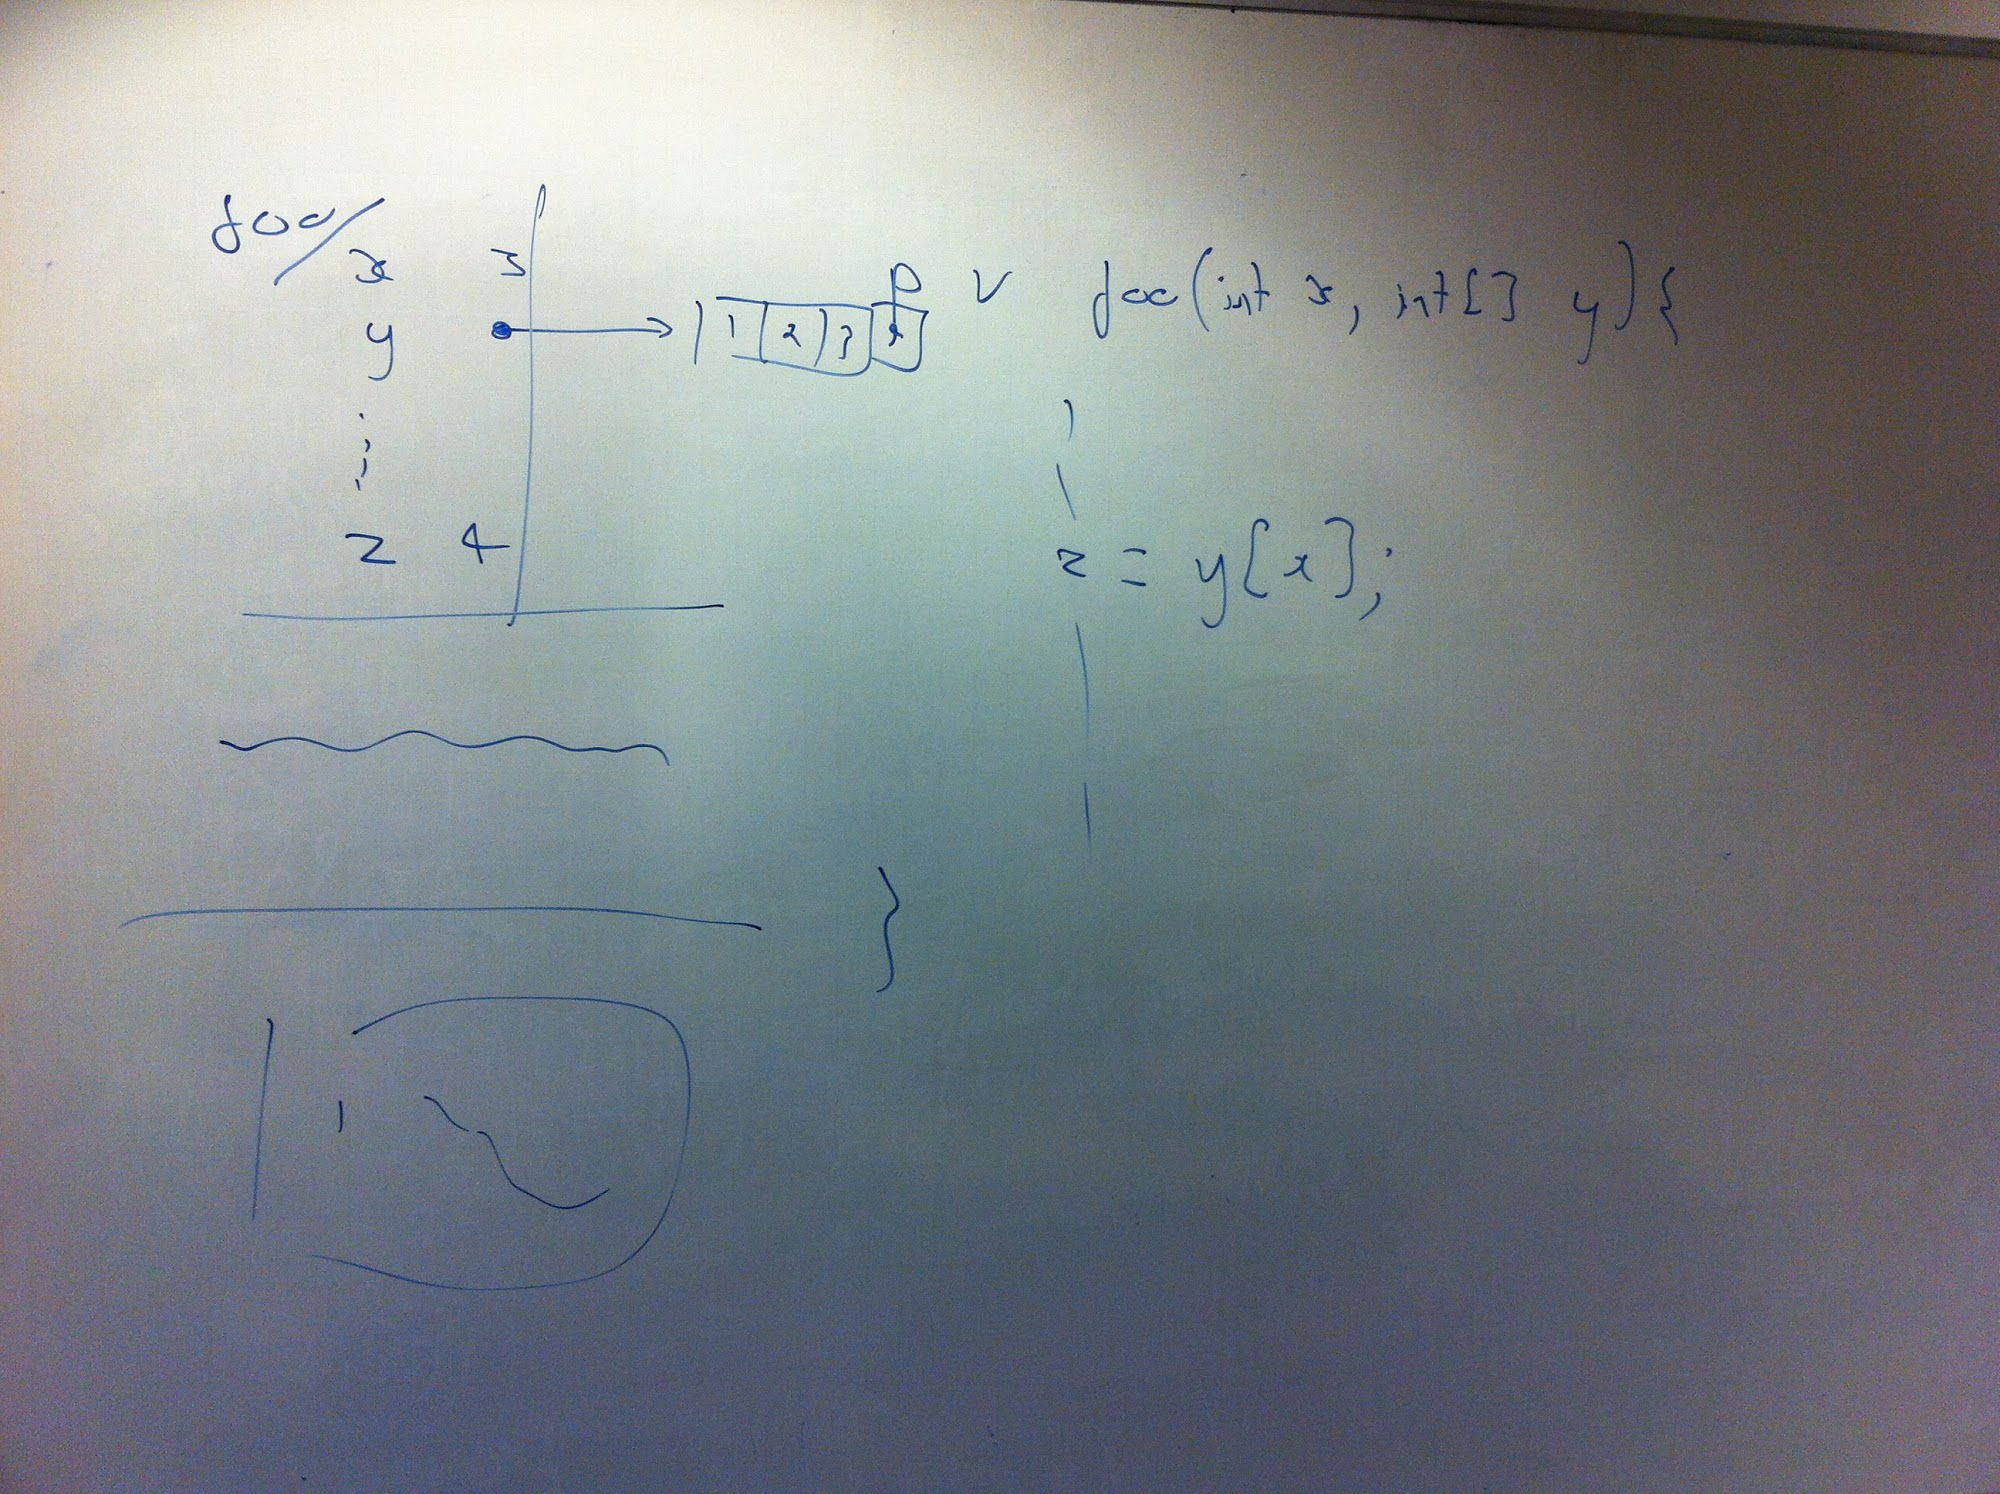
\includegraphics[width=\textwidth]{sketch.jpg}
\end{figure}

We typically did this on a whiteboard in meetings with Tristan which we then photographed and then transitioned into a Google Docs diagram.

To avoid the costly mistake of spending a lot of time building something that we may have to throw away we mocked up our designs for the front end before creating them.
\begin{figure}[h!]
\centering
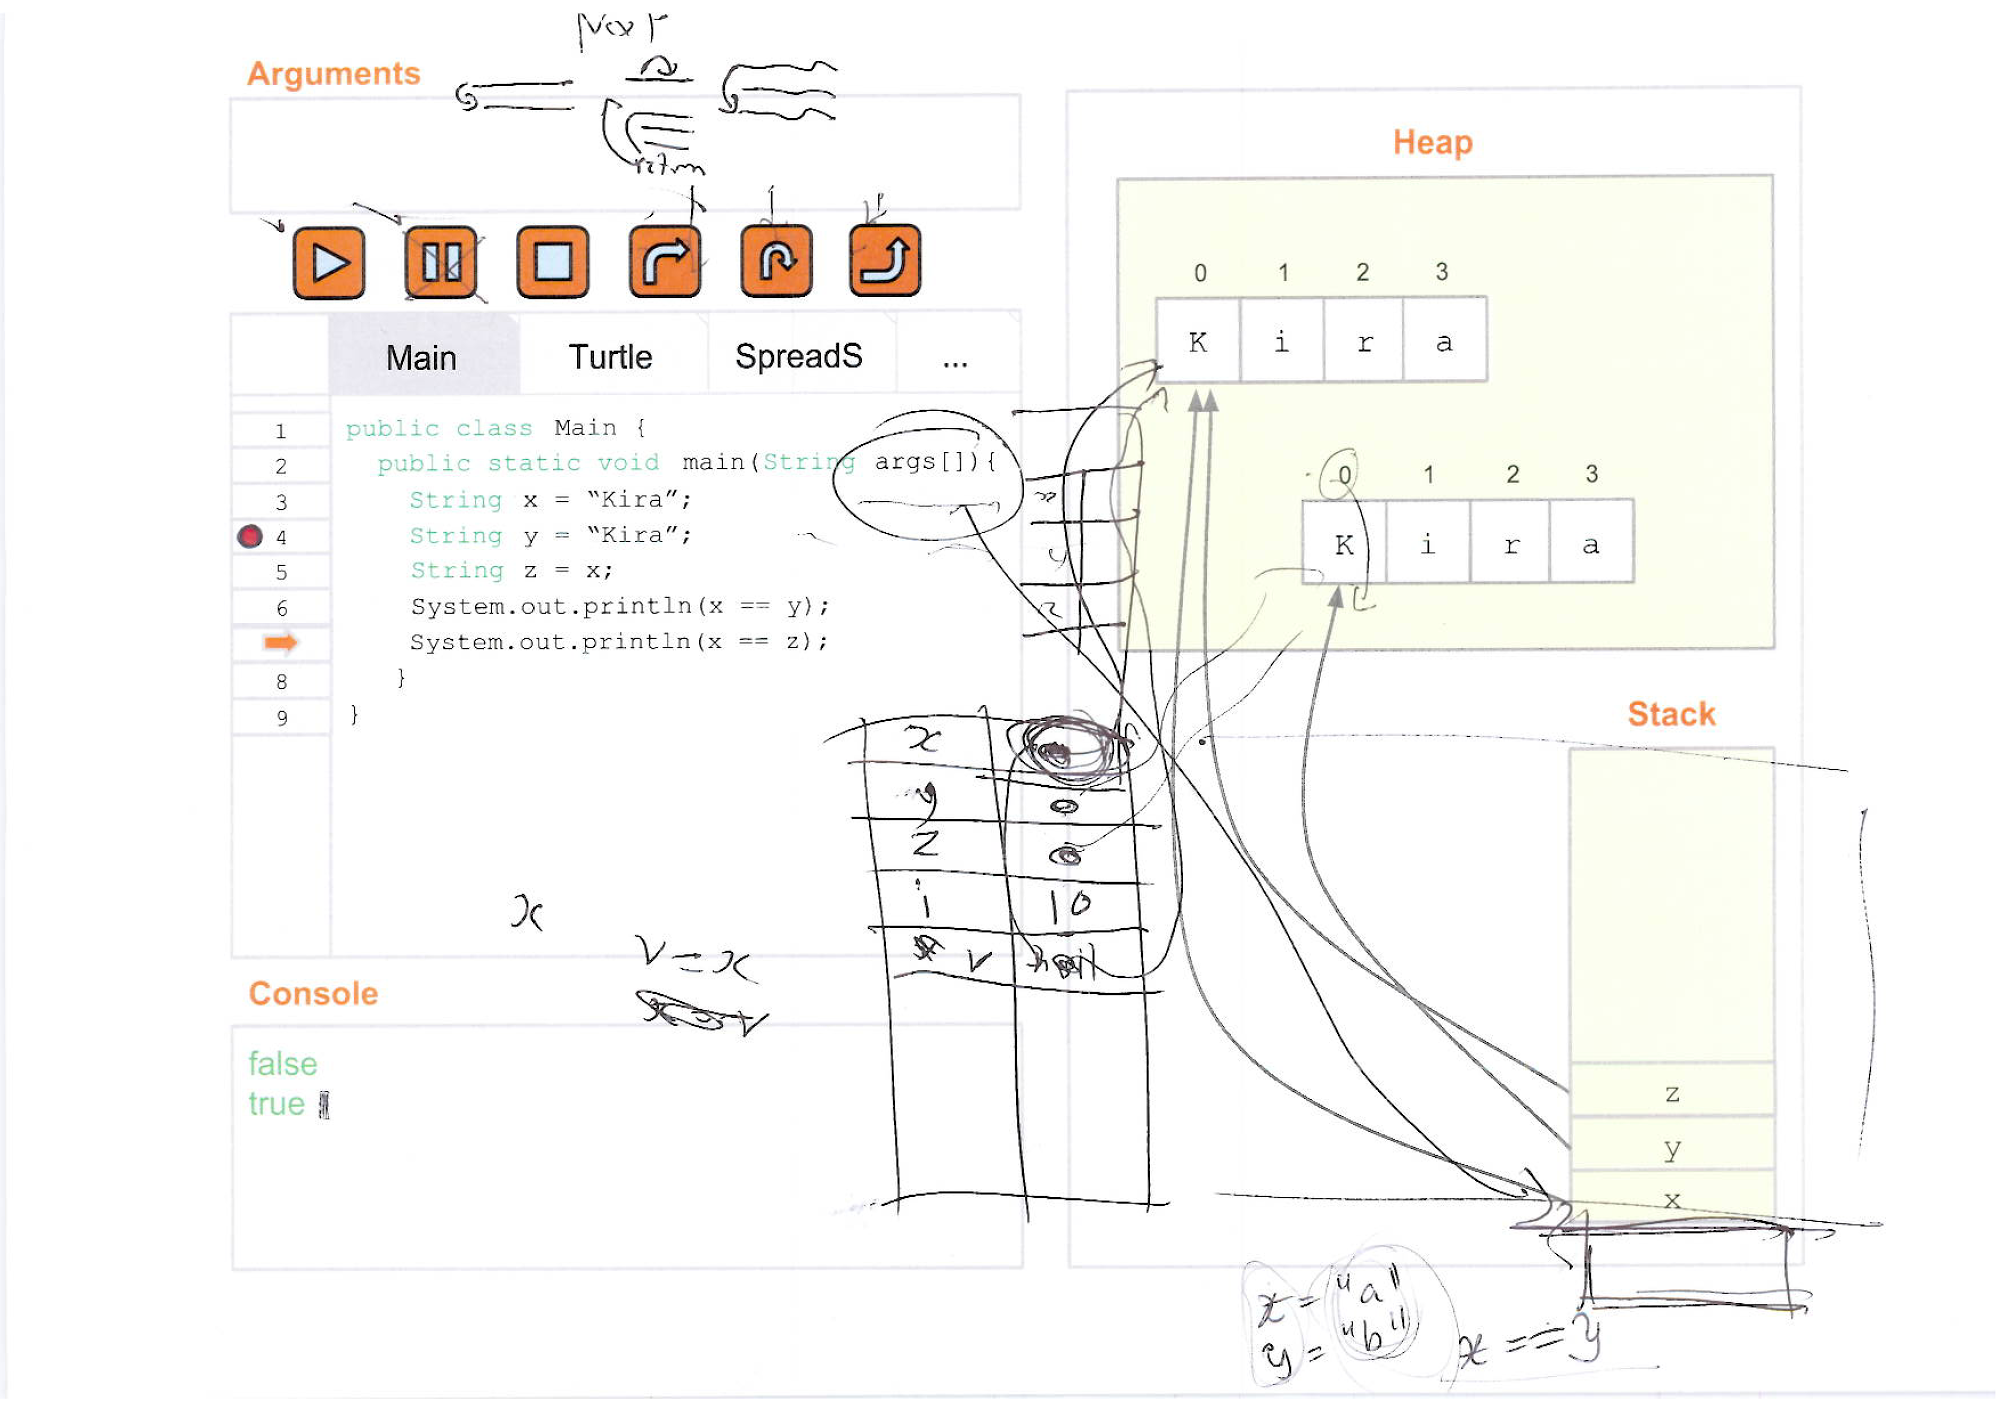
\includegraphics[width=\textwidth]{mockup.png}
\end{figure}

It then becomes easy to change and to show to first years and others for feedback. 
This does not solve every problem.
For example (as mentioned) we completed a version that was generally agreed to be good on paper and we tried it out in a lecture hall and found that the text was not readable from the back.
We have fixed our process to avoid this problem in the future, from now on after mocking in Google Docs we can test the mock at the expected size in the lecture hall.
\subsection{Frontend Design}
\subsubsection{Overview}

\subsubsection{UI Design}
\begin{figure}[h!]
\centering
\subfigure[First UI Design]{%
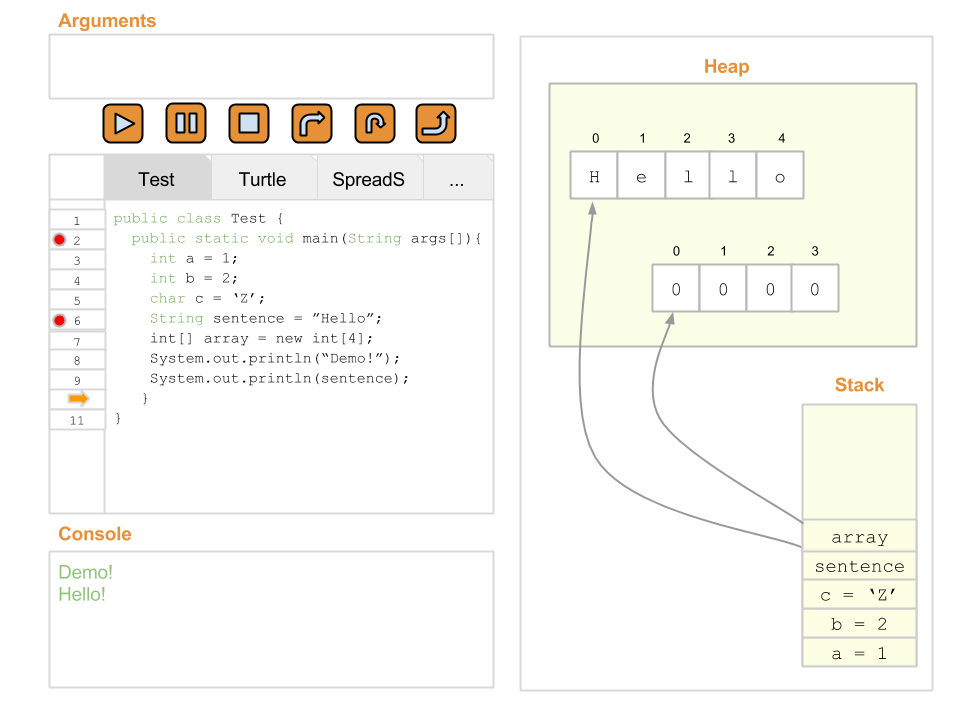
\includegraphics[height=70mm, width=60mm]{designIdea1.png}}
\quad
\subfigure[Second UI Design]{%
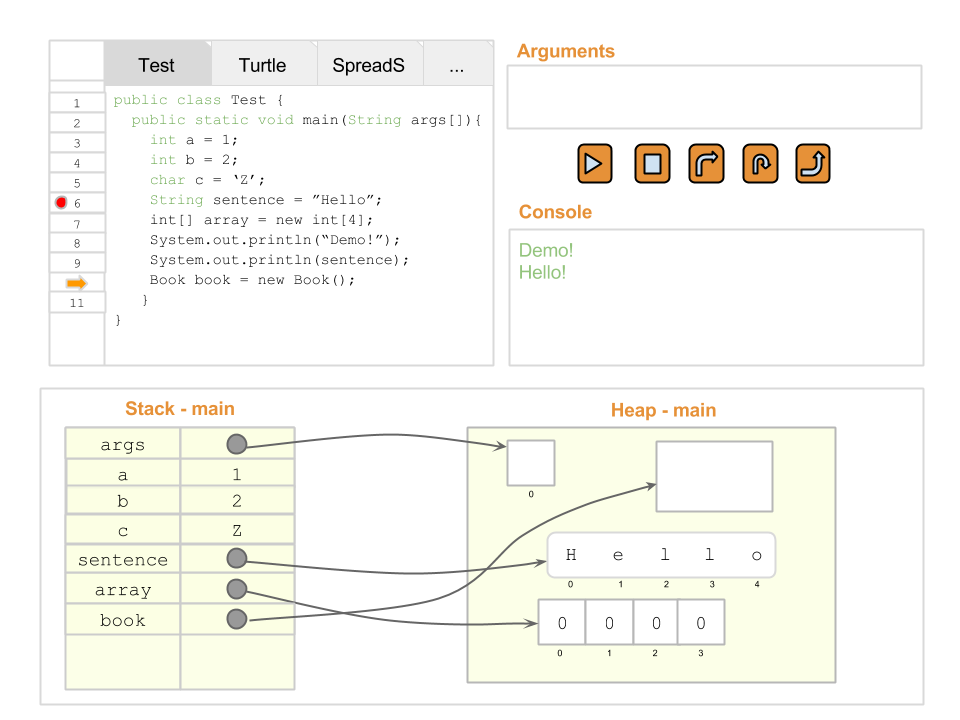
\includegraphics[height=70mm, width=60mm]{designIdea2.png}}
\end{figure}

Initially, we designed different views of the UI where the stack, heap and the code pane lay in different order.
After talking to Tristan, we thought if we put the stack and the heap visual at the bottom instead of on the right, we could better manage scenarios like small screens, a growing stack and large arrays.
As a result, we modified our UI design to be similar to the picture on the right above.\\
\begin{figure}[h!]
\centering
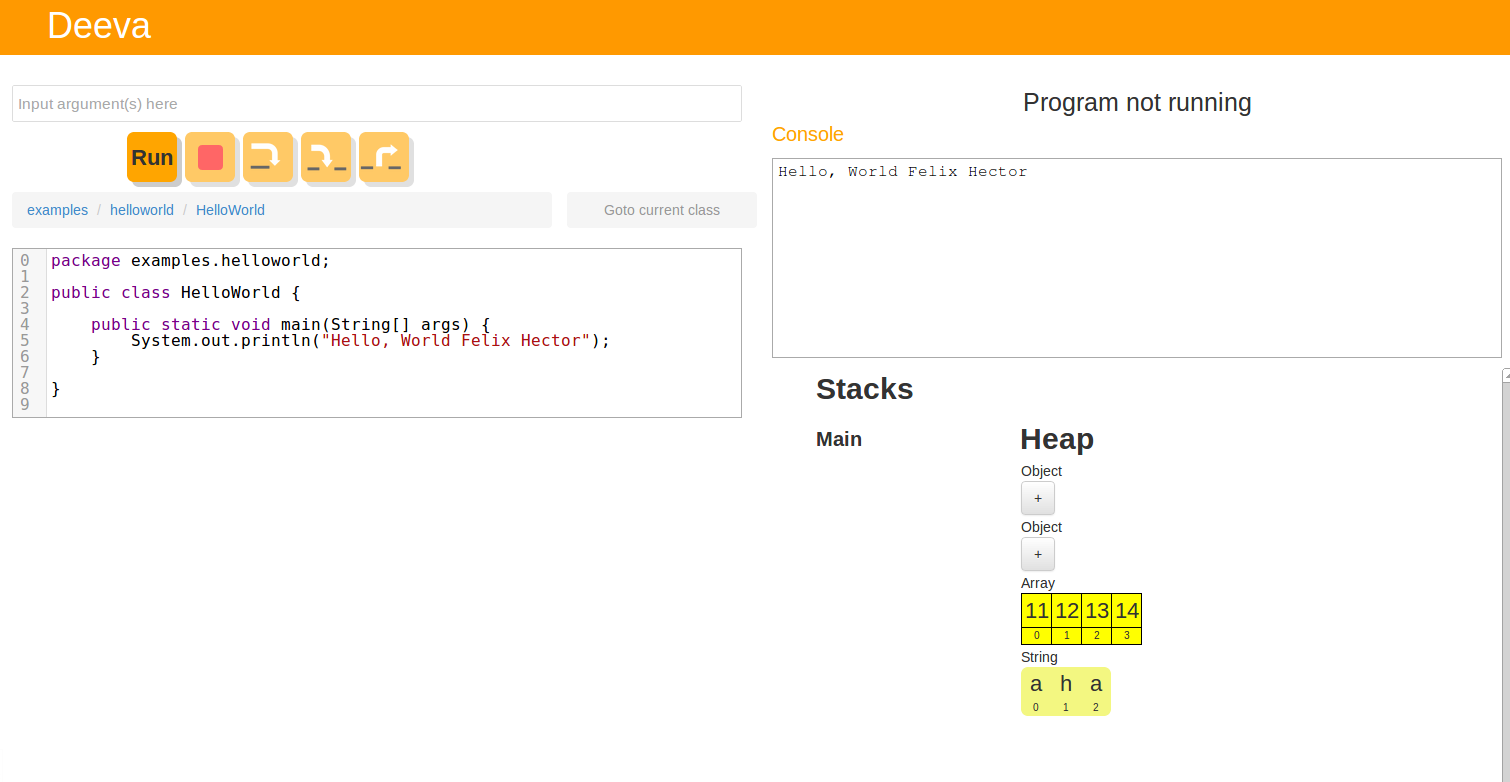
\includegraphics[height=70mm,width=130mm]{finalDesign.png}
\end{figure}

However, we thought if the stack grow more then eventually user would need to scroll up and down to be able to see the code and the stack and heap at the same time, which is not really what we want.
Therefore, we agreed on putting the stack and heap on the right with some modification to the first design.

\subsubsection{Button Design}
After conducting some interviews with users (see ~\cref{sec:evaluation}), we discovered that some people found the naming and the design of buttons very confusing in Eclipse.
Especially the ``Step Into'', ``Step Over'' and ``Step Return'' buttons which control movement through the code.
As a result, we designed several different sets of buttons and used a questionnaire to pick among them.

\begin{figure}[h!]
\centering

\includegraphics[height=20mm,width=60mm]{buttons1.png}
\caption{Initial Design of the ``Stepping'' Buttons}
\end{figure}

This is our original design of the ``Stepping'' buttons.
They inherit the design from the Eclipse debugger.
They are \cmd{Step Into}, \cmd{Step Over} and \cmd{Step Return} from left to right respectively.

\begin{framed}
\emph{A digression on the behavior of the Stepping buttons.}

\begin{description}
\item Step Into
\item Step Over
\item Step Return
\end{description}

\end{framed}


We asked a friend who does not study Computing and who has not used a debugger before but has had exposure to programming before what he guessed each one should do.
He could not quite figure it out just by looking at them confirming our suspicion that these are not the most intuitive of designs.
We then explained the concept of \cmd{Step Into}, \cmd{Step Over} and \cmd{Step Return} in terms of debugging and then asked again if he thought any of them really matched the buttons.\todo{edit}
He gave us some valuable feedback: ``It would be useful if we could somehow represent different scopes/lines so that the arrows (along with their direction) can correctly express the intended function.''
\begin{figure}[h!]
\centering

\includegraphics[height=20mm,width=60mm]{buttons2.png}
\caption{Redesign of the ``Stepping'' Buttons}
\end{figure}

This is our second design.
As suggested by our friend, the black lines indicate the lines of code which is similar to an editor.
Arrows going in either the upwards or downwards directions indicate going to the next line, function, or (or previous) scope.
We created a questionnaire in which we explained the definition of ``Next", ``Into" and ``Out" (our new and hopefully more intuitive names for the functionality previously known as ``Step Into'', ``Step Over'' and ``Step Return'').

Then we asked which of the eight button designs best represents the aforementioned functions.
We gave out the questionnaires (see ~\cref{sec:buttonquestionnaire}) when we did the Hallway Testing (see ~\cref{sec:evaluation}) to some first year students and second year students.
Our second set of designs were much more popular than the original design among first year students.
However most of the second year students chose the original Eclipse design, one of them explaining that because they had already used Eclipse they were used to the original buttons.

In the end we did not use the second design because of some confusion from our users and comments from our project supervisor during the process. 
It was not that clear what the black lines indicate especially for experienced users who are already used to the original design common to many debuggers additionally given that we expect users to graduate to using the Eclipse and other debuggers we did not want to create a whole new design vocabulary that they would soon have to relearn. 
We did however keep the new more intuitive names.

\subsubsection{Colour Scheme and Font Size Design}
We carried out a test and questionnaire in front of a first year Java class to see which colour scheme and font size are the most liked and most visible on the projector in the lecture hall.

\begin{figure}[h!]
\centering
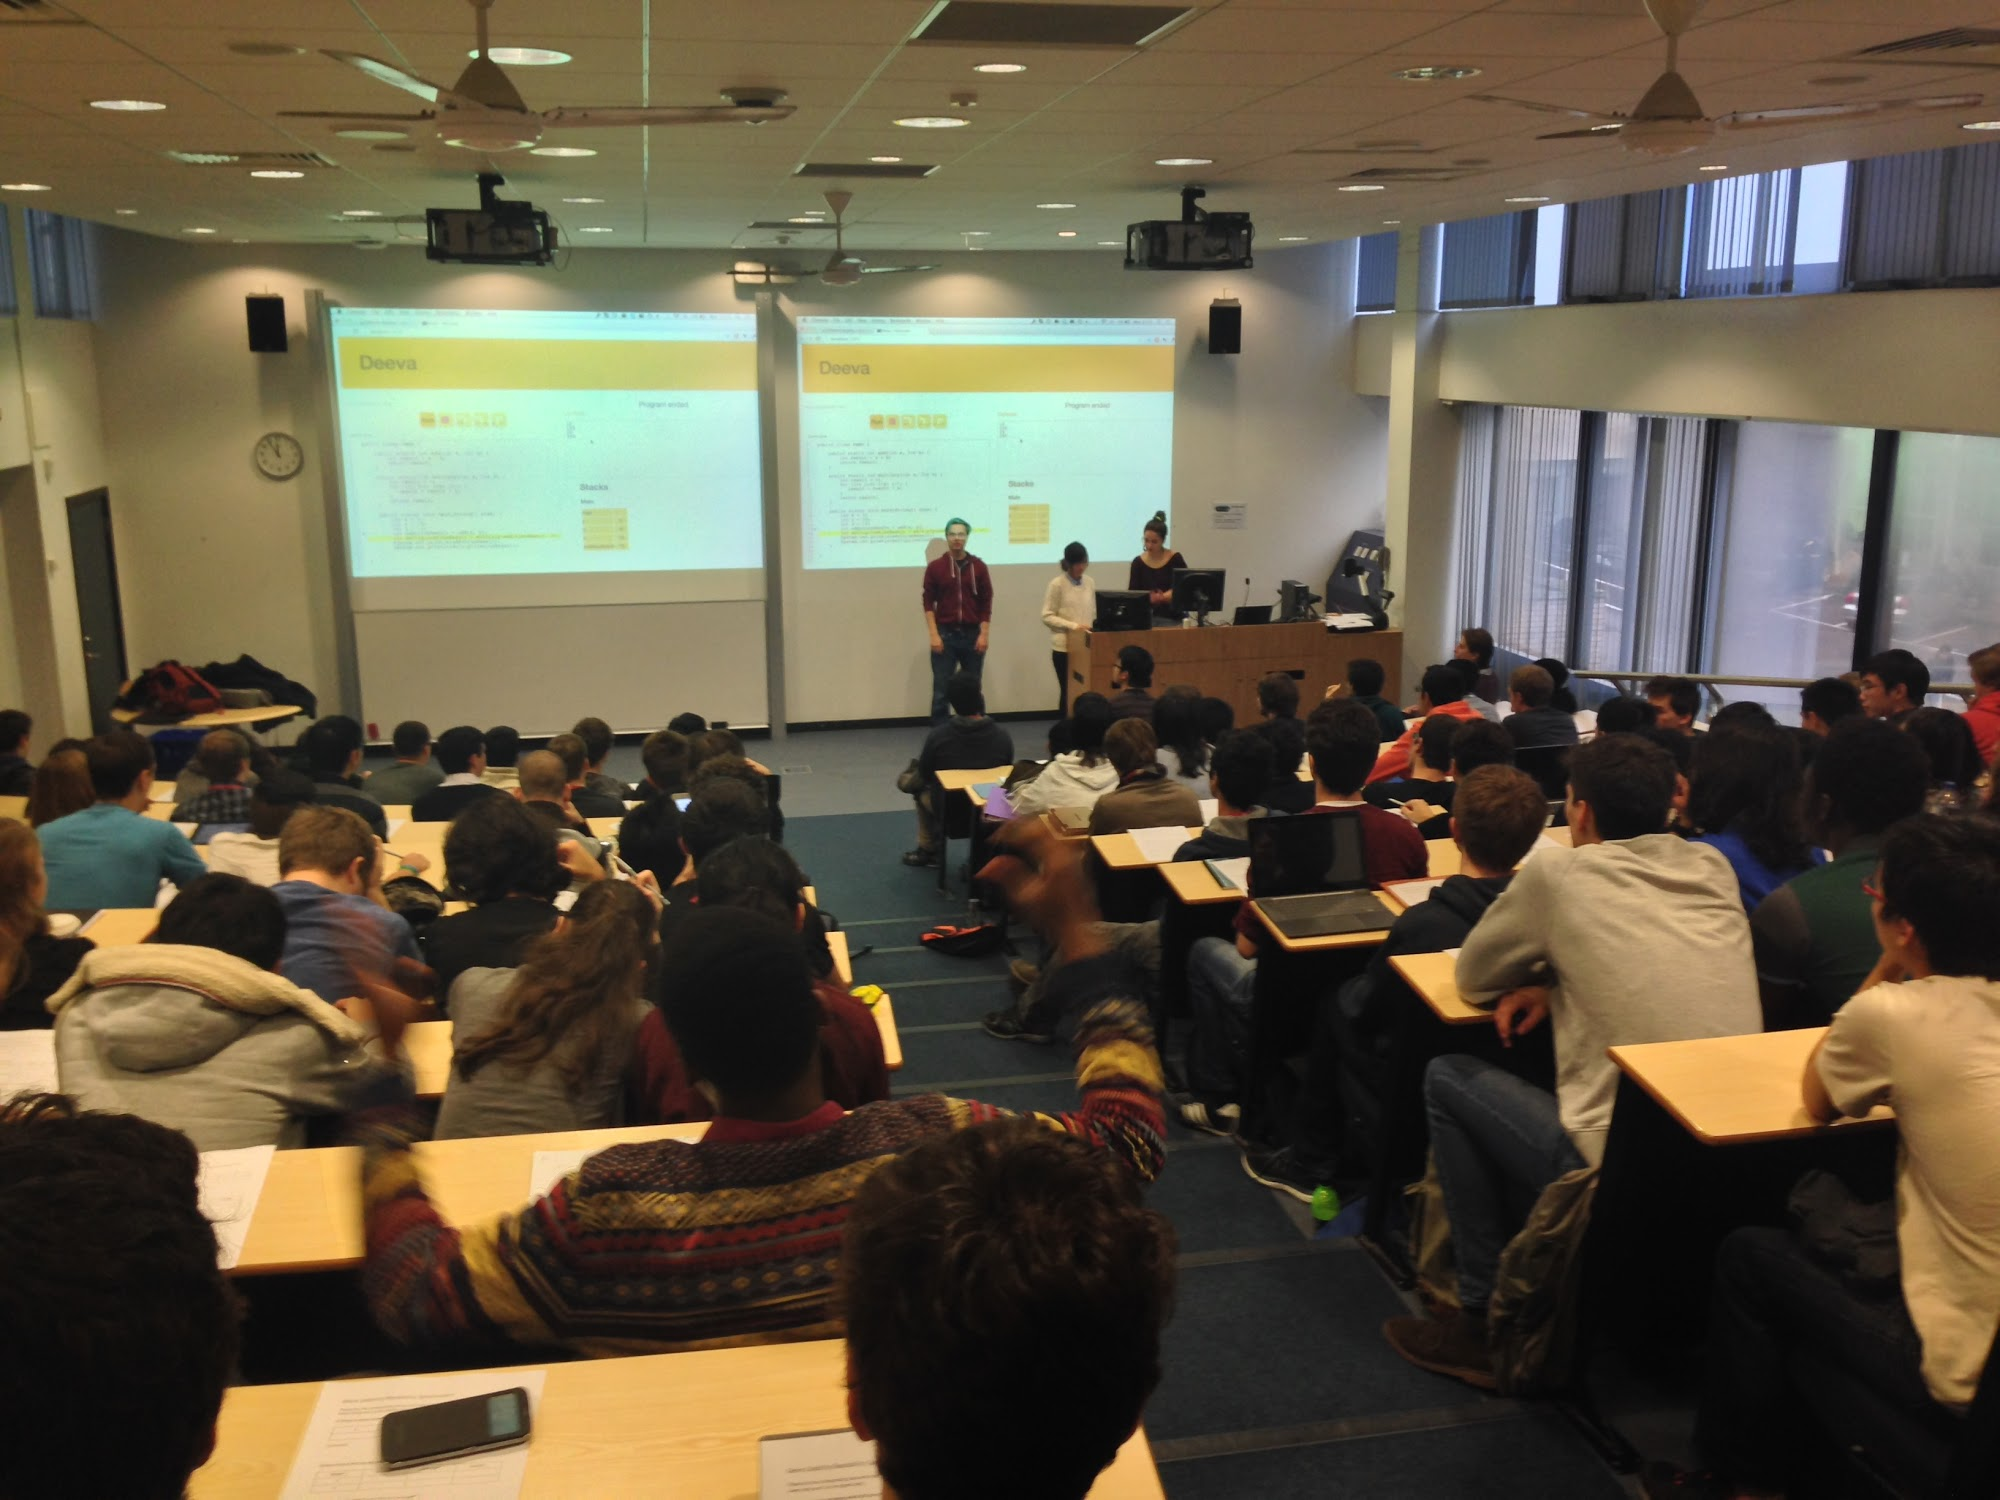
\includegraphics[height=50mm,width=100mm]{lectureHall.jpg}
\caption{Font size and colourscheme test in first year lecture.}
\end{figure}

Given 5 different colour schemes, the preferred choice was our current colour scheme (orange), followed by a light blue color scheme (see graph on the right).
This validated our initial research that showed that in visual presentations, people are attracted to bright, warm colours that express optimism.
\begin{figure}[h!]
\centering
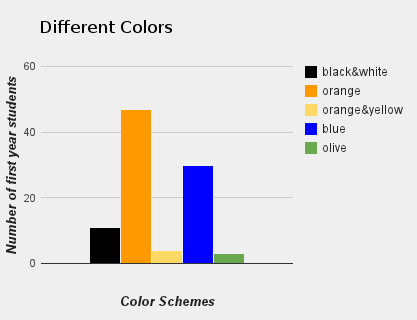
\includegraphics[height=60mm,width=100mm]{colours.png}
\end{figure}

As some people expressed that they would like the possibility to personalise Deeva and have a choice between different colour schemes we included this feature on the extended list of features for our final product.

However, this is not a priority as we are more concerned with implementing more functionality rather than a personalised UI design.

For font size, we provided 2 samples on the projector screen.
Sample 1 had a font size of 26px and Sample 2 had a font size of 16px.
\begin{figure}[h!]
\centering
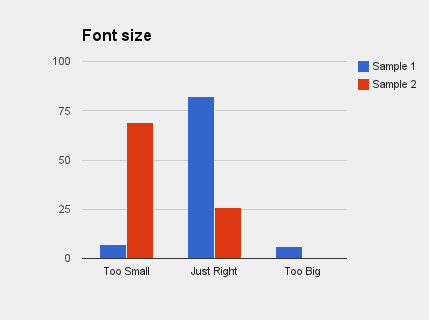
\includegraphics[height=60mm,width=100mm]{fonts.png}
\end{figure}
As this questionnaire was performed in one of the big lecture rooms (Huxley 311) the results for this question did not surprise us, people preferred the sample with the bigger font size (see graph on the right).
However, as the smaller font size sample is perfectly readable on the lab machines we are thinking\todo{fix} of releasing our debugger in two modes: `normal mode' (to be used on the lab machines - font size 16) and  `lecturer mode' (to be used by lecturers when teaching - font size 26).
This was not part of our initial plan so, consulting with our project supervisor, we amended our list of extensions adding a `lecturer mode' to the top.

\subsection{System Design}

\section{Implementation}
\subsection{Technology Evaluation}
\subsection{Overview}
\subsection{Details}
\subsubsection{Front End}
\subsubsection{Middleware}
\subsubsection{Back End}

\section{Evaluation}
\label{sec:evaluation}
We used a number of techniques to evaluate Deeva.
We used some techniques to help us find or fix specific problems and we used others to make sure that we were on the right track building the right things.
\subsection{Usibility Testing}

\subsubsection{Hallway Testing}
\begin{figure}[h!]
\centering
\subfigure{%
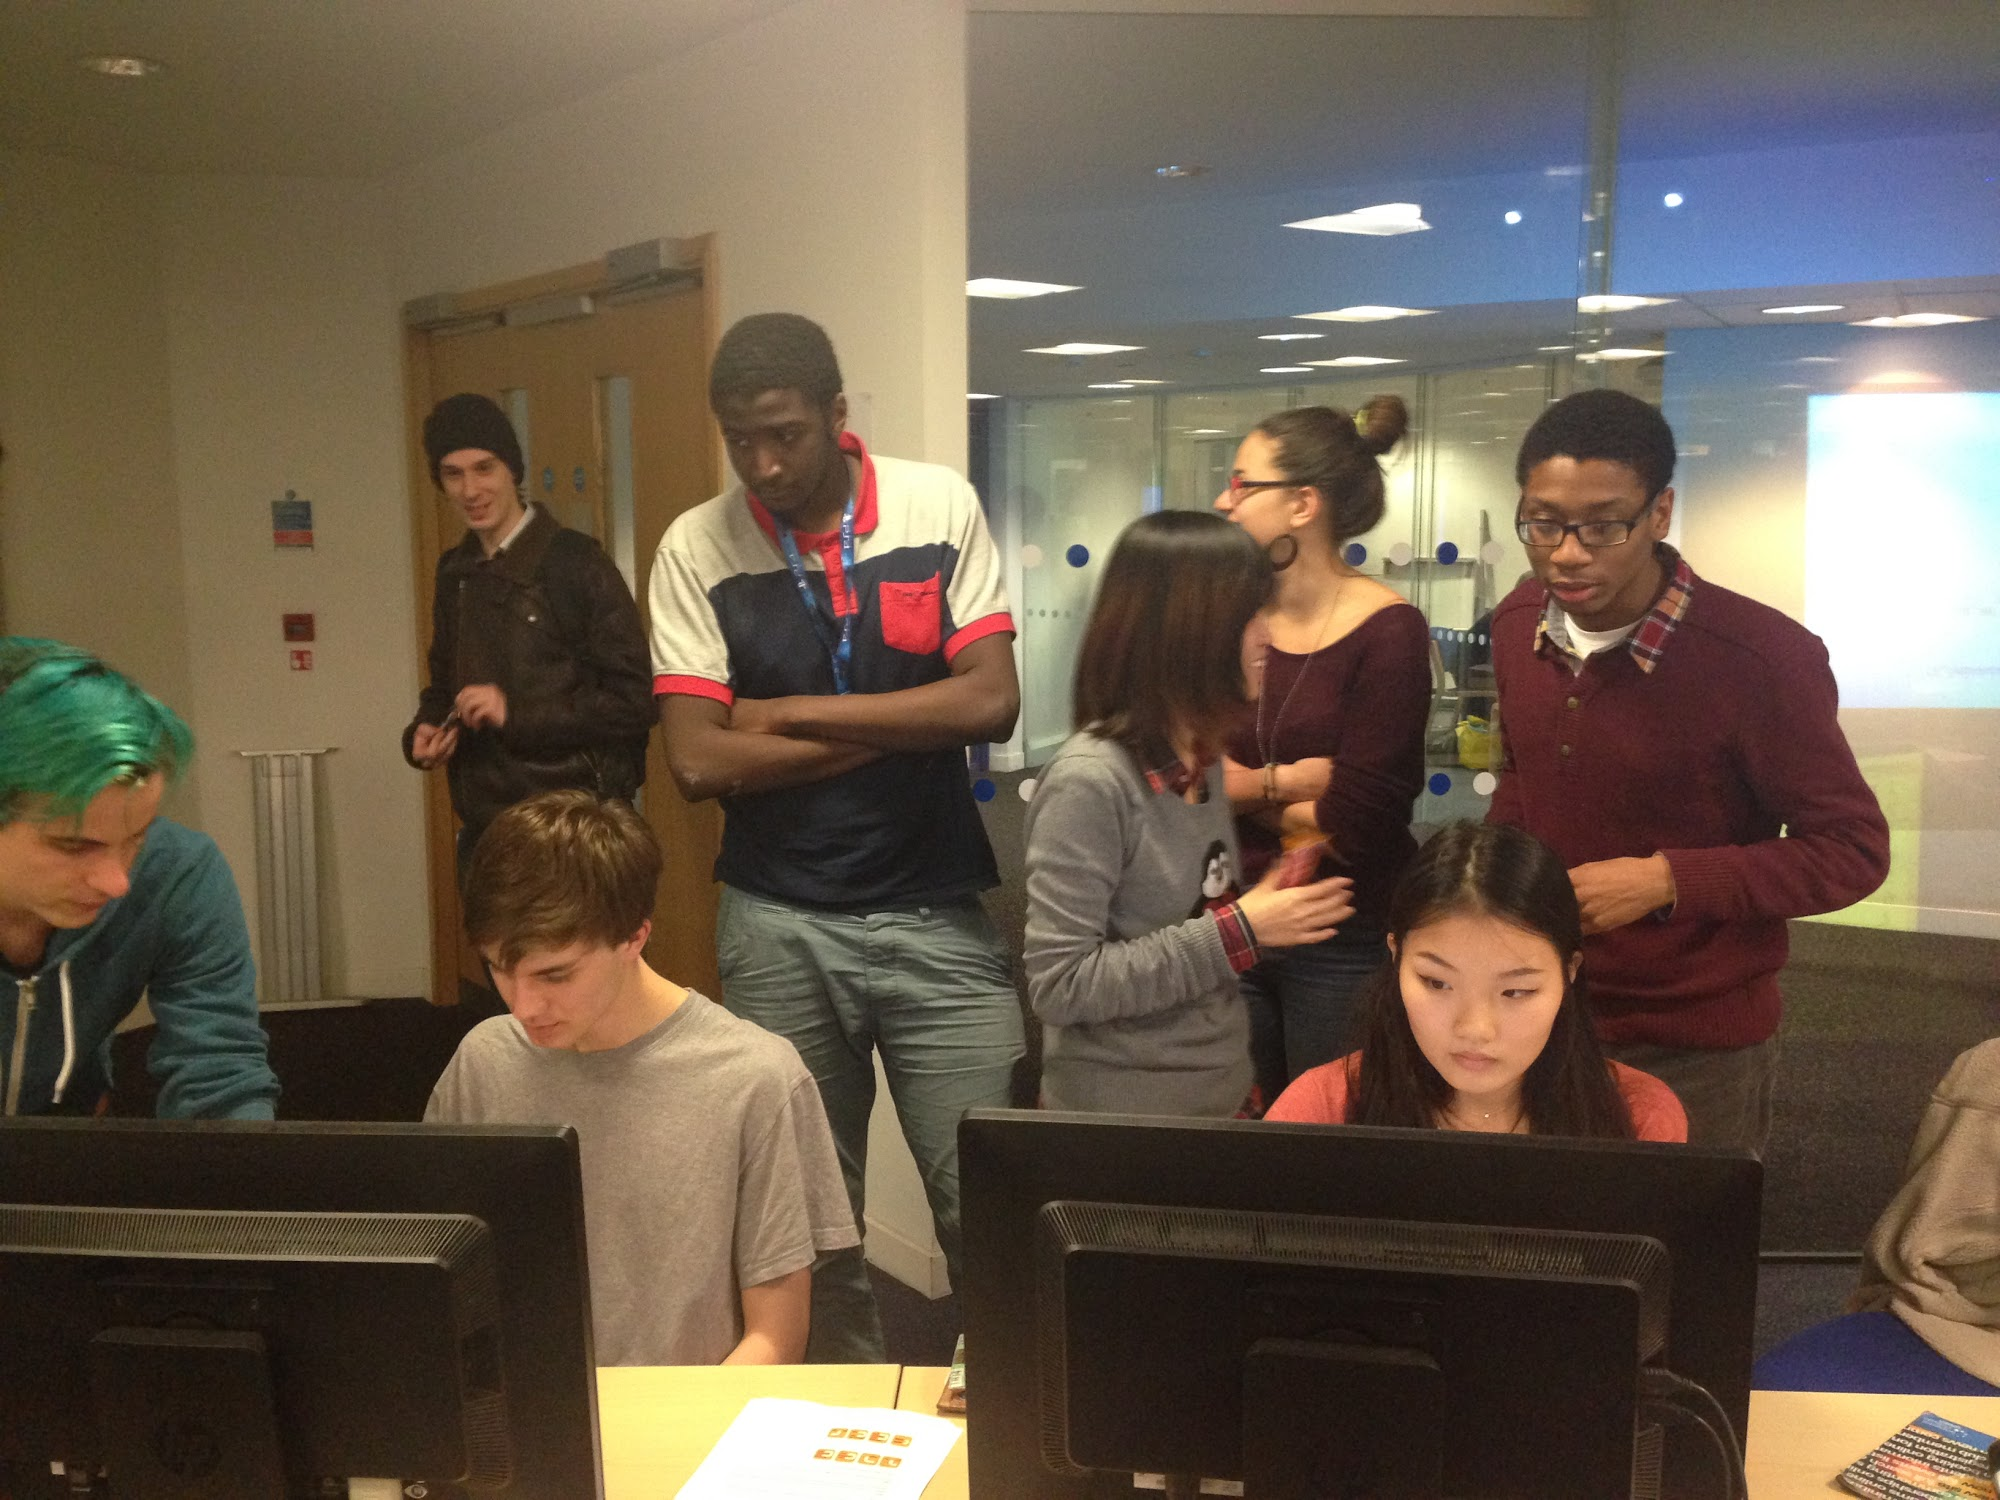
\includegraphics[height=50mm, width=60mm]{hallway1.jpg}}
\quad
\subfigure{%
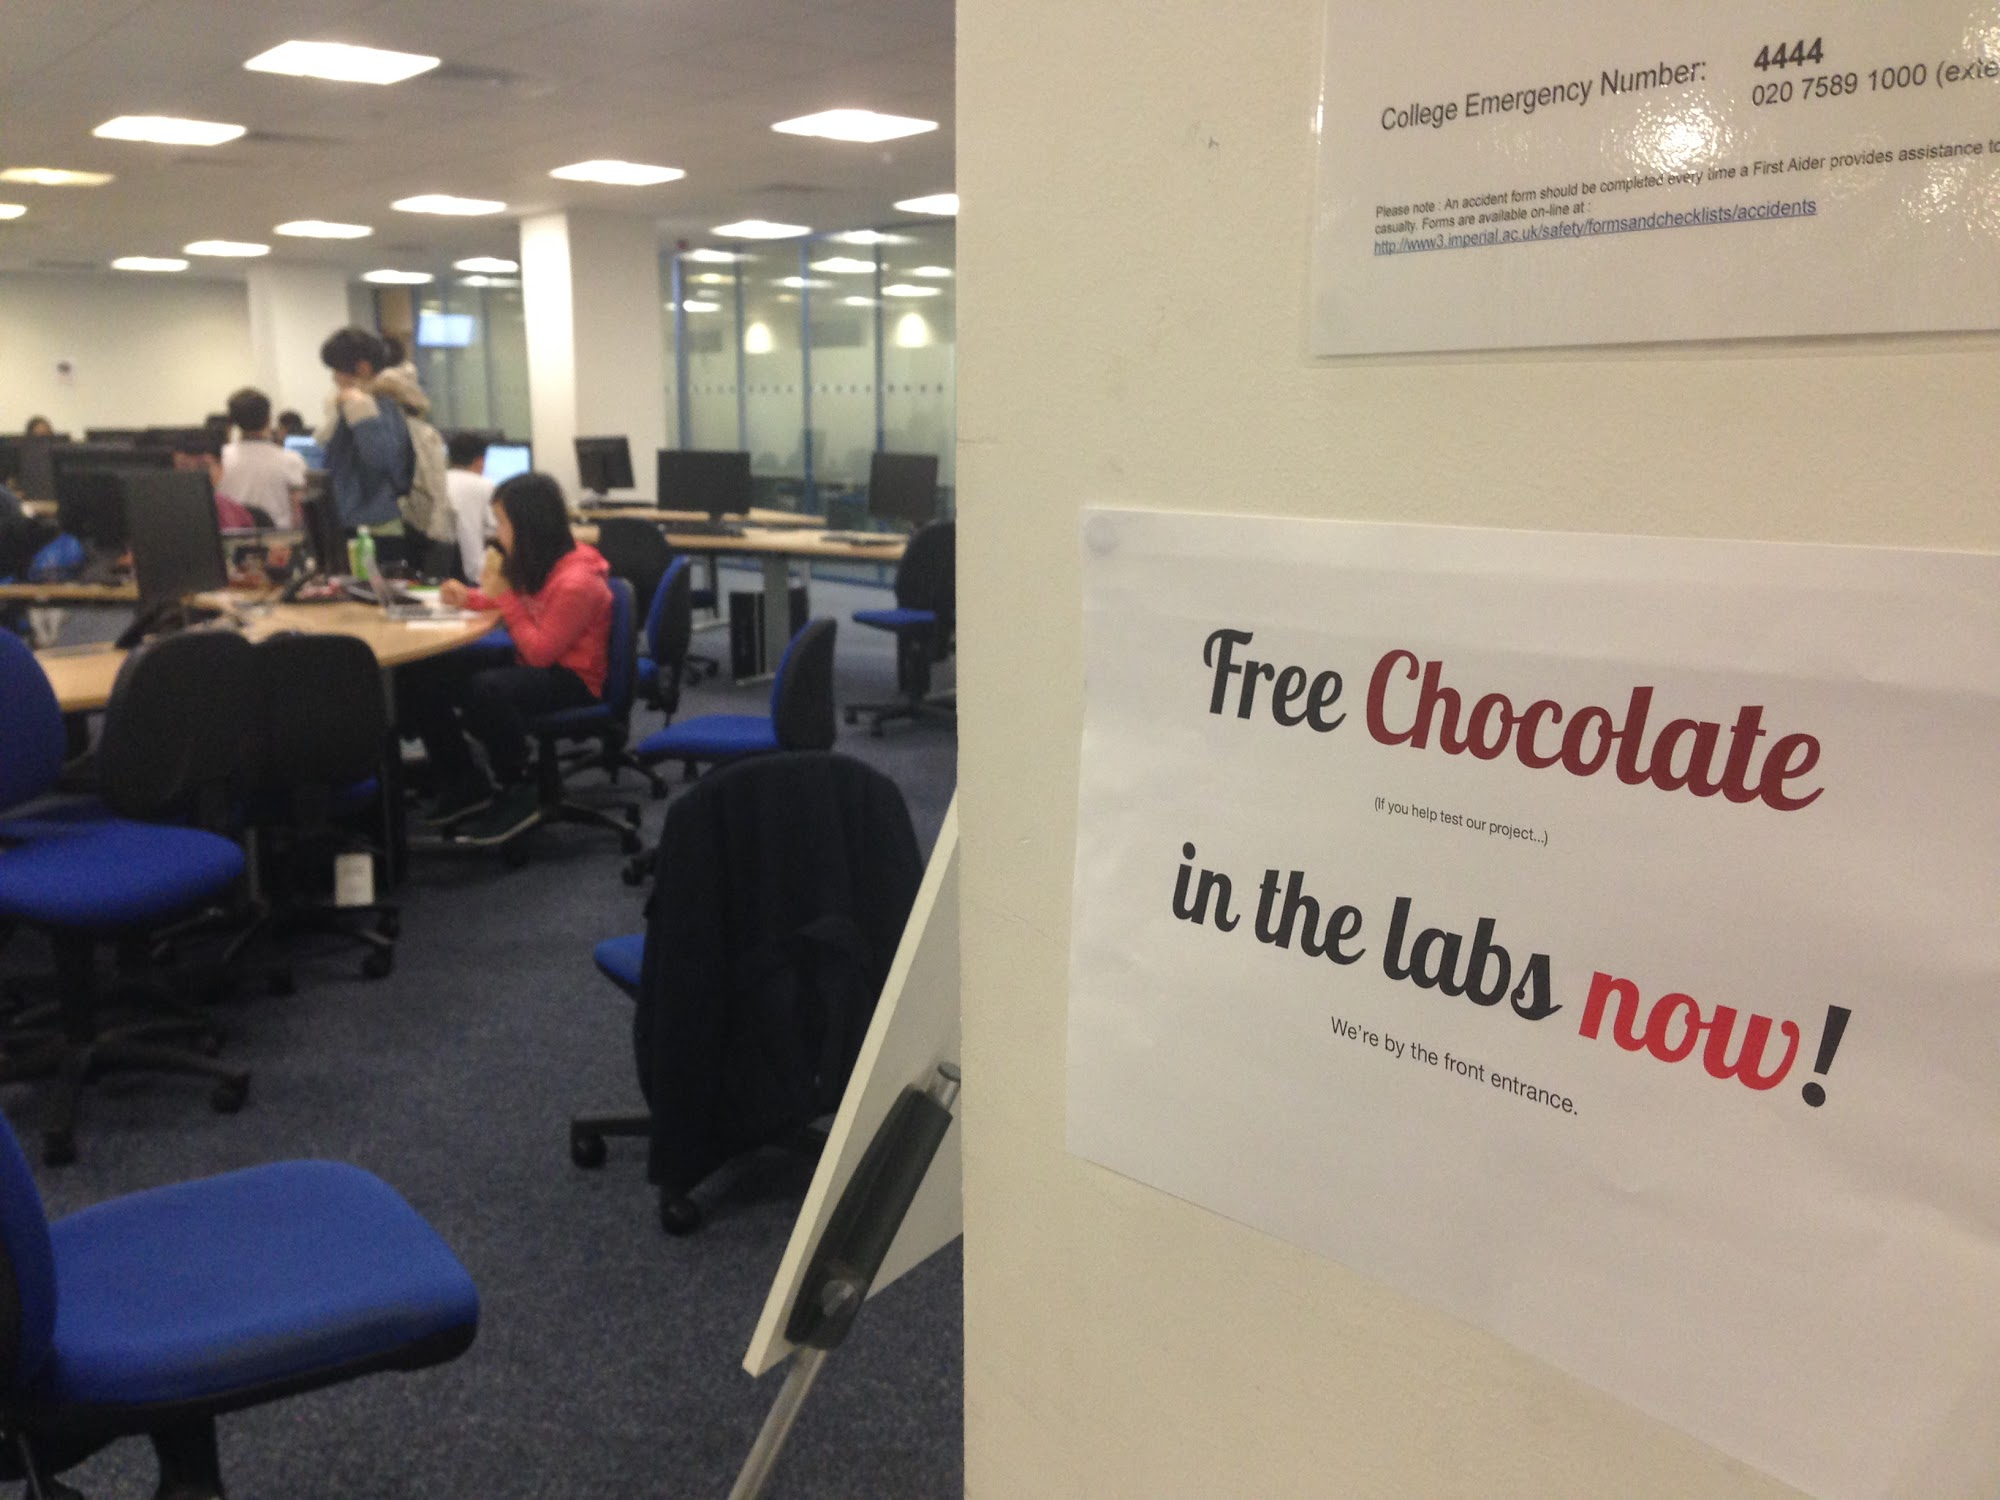
\includegraphics[height=50mm, width=60mm]{hallway2.jpg}}
\end{figure}

We employed a hallway testing approach when it came to evaluating the usability of our debugger, by getting the first year students (our primary stakeholders) and some second year students to demo our project and tell us their first impressions and what they were expecting. This was beneficial because as the developers, we are aware of the caveats and may subliminally navigate around them.
Using the feedback from first year students allowed us to identify critical bugs/pitfalls in our usability design.
This was obviously more qualitative however we used some measures (like how many times they had to ask questions) to help quantify things such as how intuitive the interface was or feature complete it was.
On average, the people who participated in the testing asked around 1-3 questions related to basic features like how to run Deeva or how to set a breakpoint.
This was insightful as we are aiming to make Deeva as intuitive as possible so we minimise the need to consult the help menu.
This helped mainly with our first use case which is students using Deeva on the lab machines.

\subsubsection{Quantified testing of colour schemes and font sizes}
We wanted to employ the use of A/B testing to assess how effective certain colour schemes and font sizes would be.
However we had to make a compromise, because the environment and number of users that we could get in one room simultaneously meant that we had to do it in one sitting i.e. we couldn’t let half the users in the room see one colour scheme and the other half see a different colour scheme.
So in the end we just conducted a poll so they could pick which colour scheme and font size they liked the best.
We did this with the help of our project supervisor (who lectures the course in which our debugger will primarily be used). 

This is helpful as it allows us to catch possible problems with readability early, which in our case may change the direction in which our solution is architected.
An example of this is that the projectors’ resolution in the lecture room is small, so not all the necessary information can be seen.
Hence, we may need to have a separate mode which shows just the stack and the heap.
The implication of this mode meant we had to change our implementation to be less monolithic.

\subsubsection{Questionnaire}
\begin{figure}[h!]
\centering
\subfigure{%
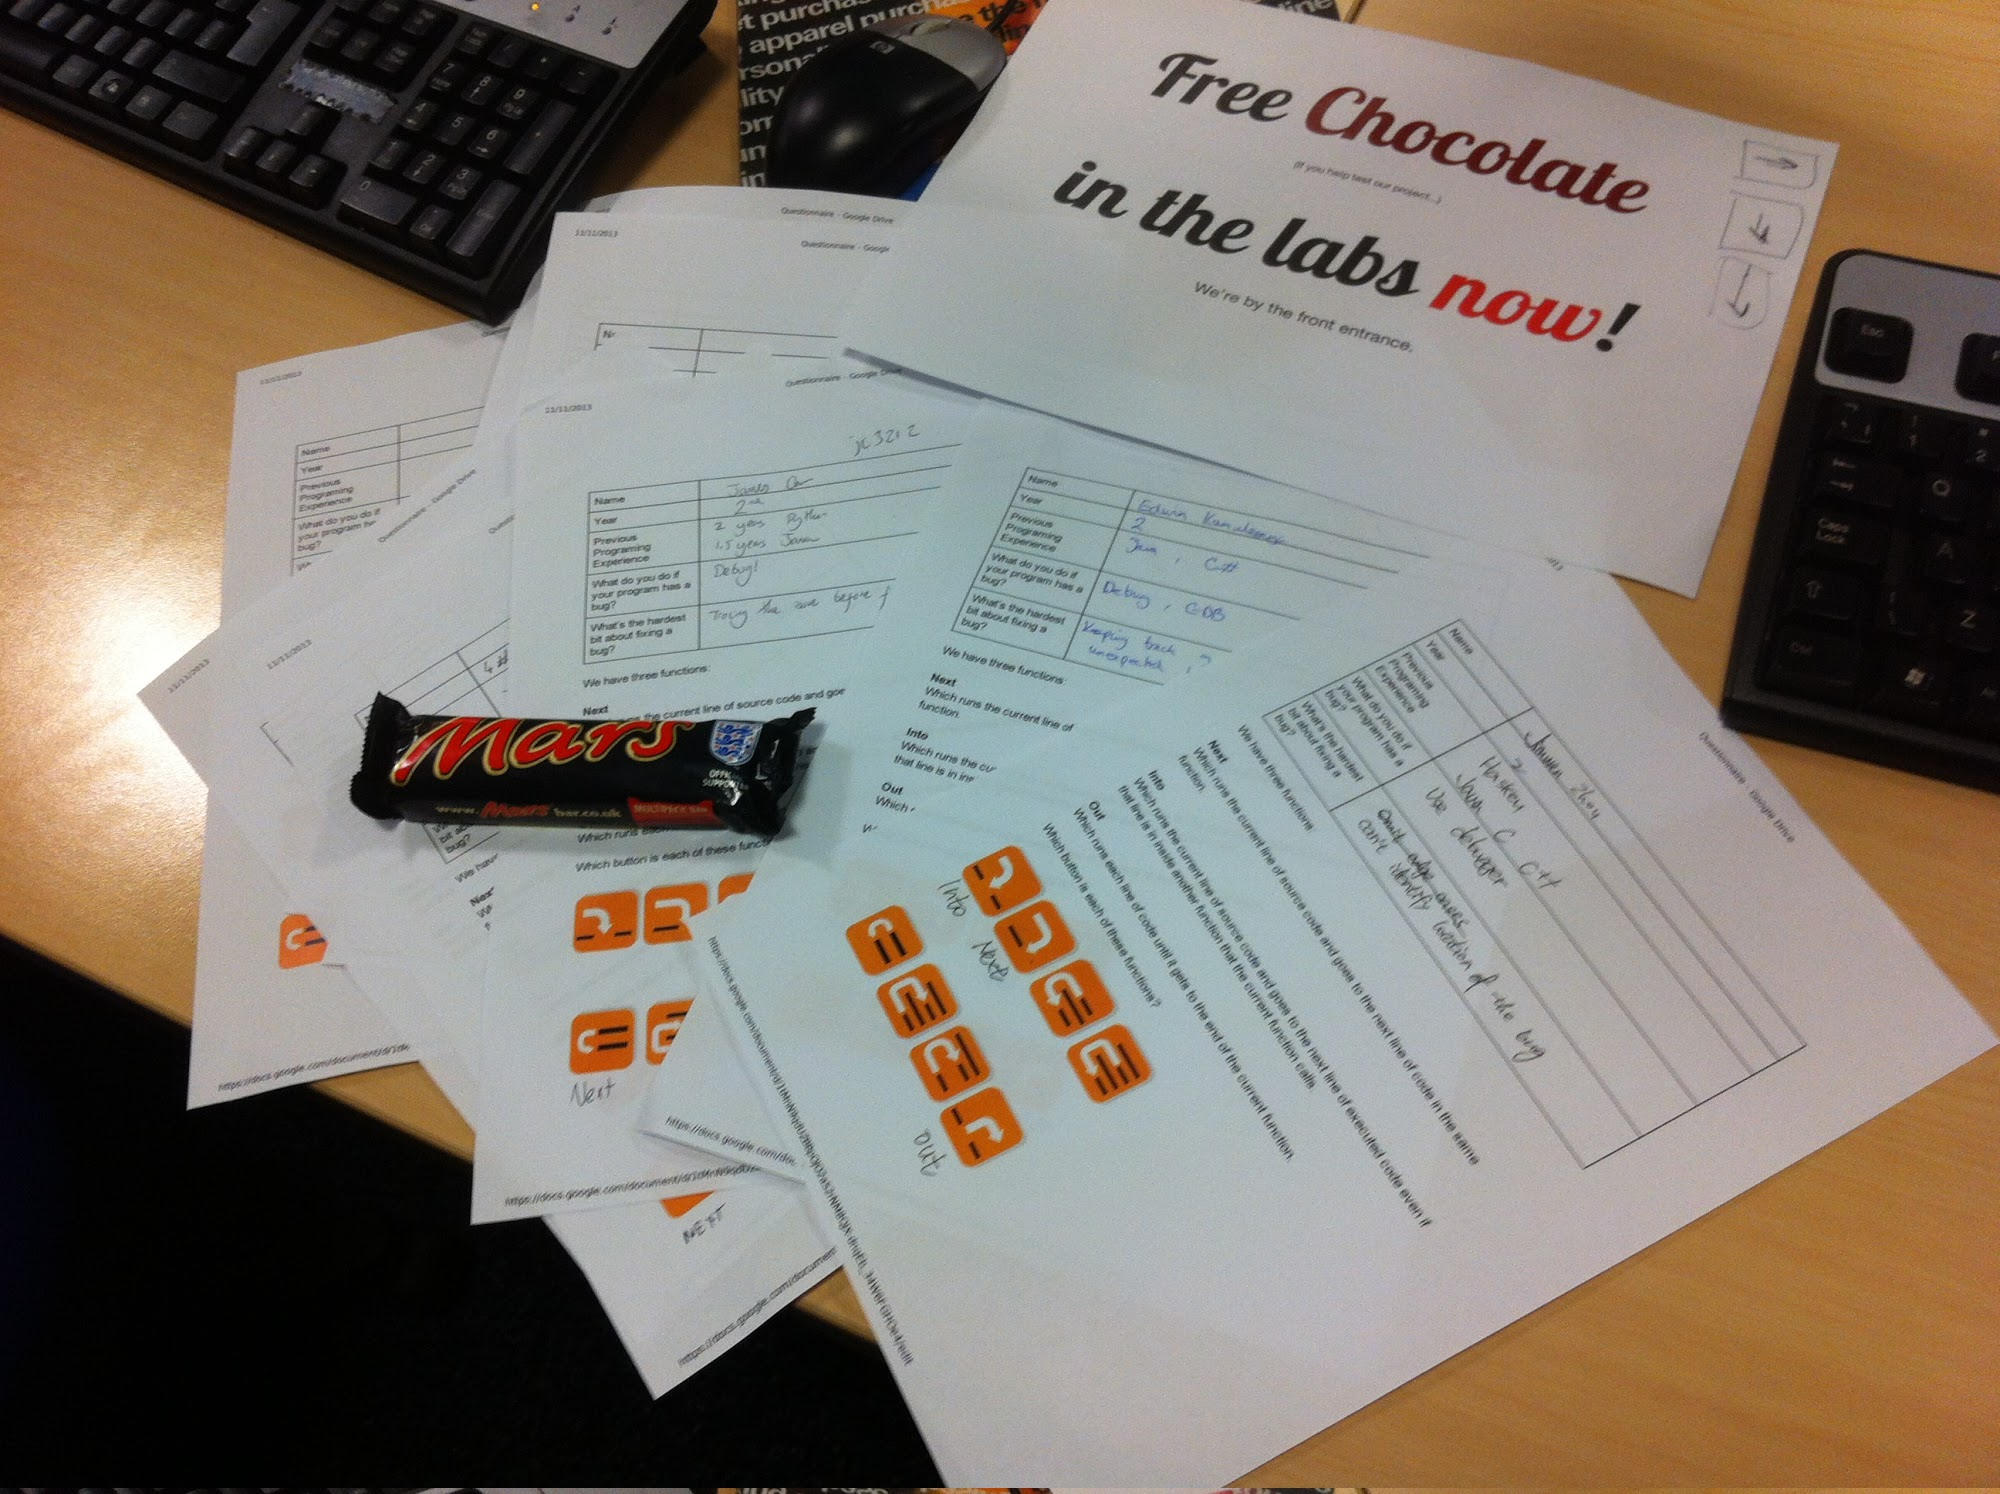
\includegraphics[height=50mm, width=60mm]{questionnair1.jpg}}
\quad
\subfigure{%
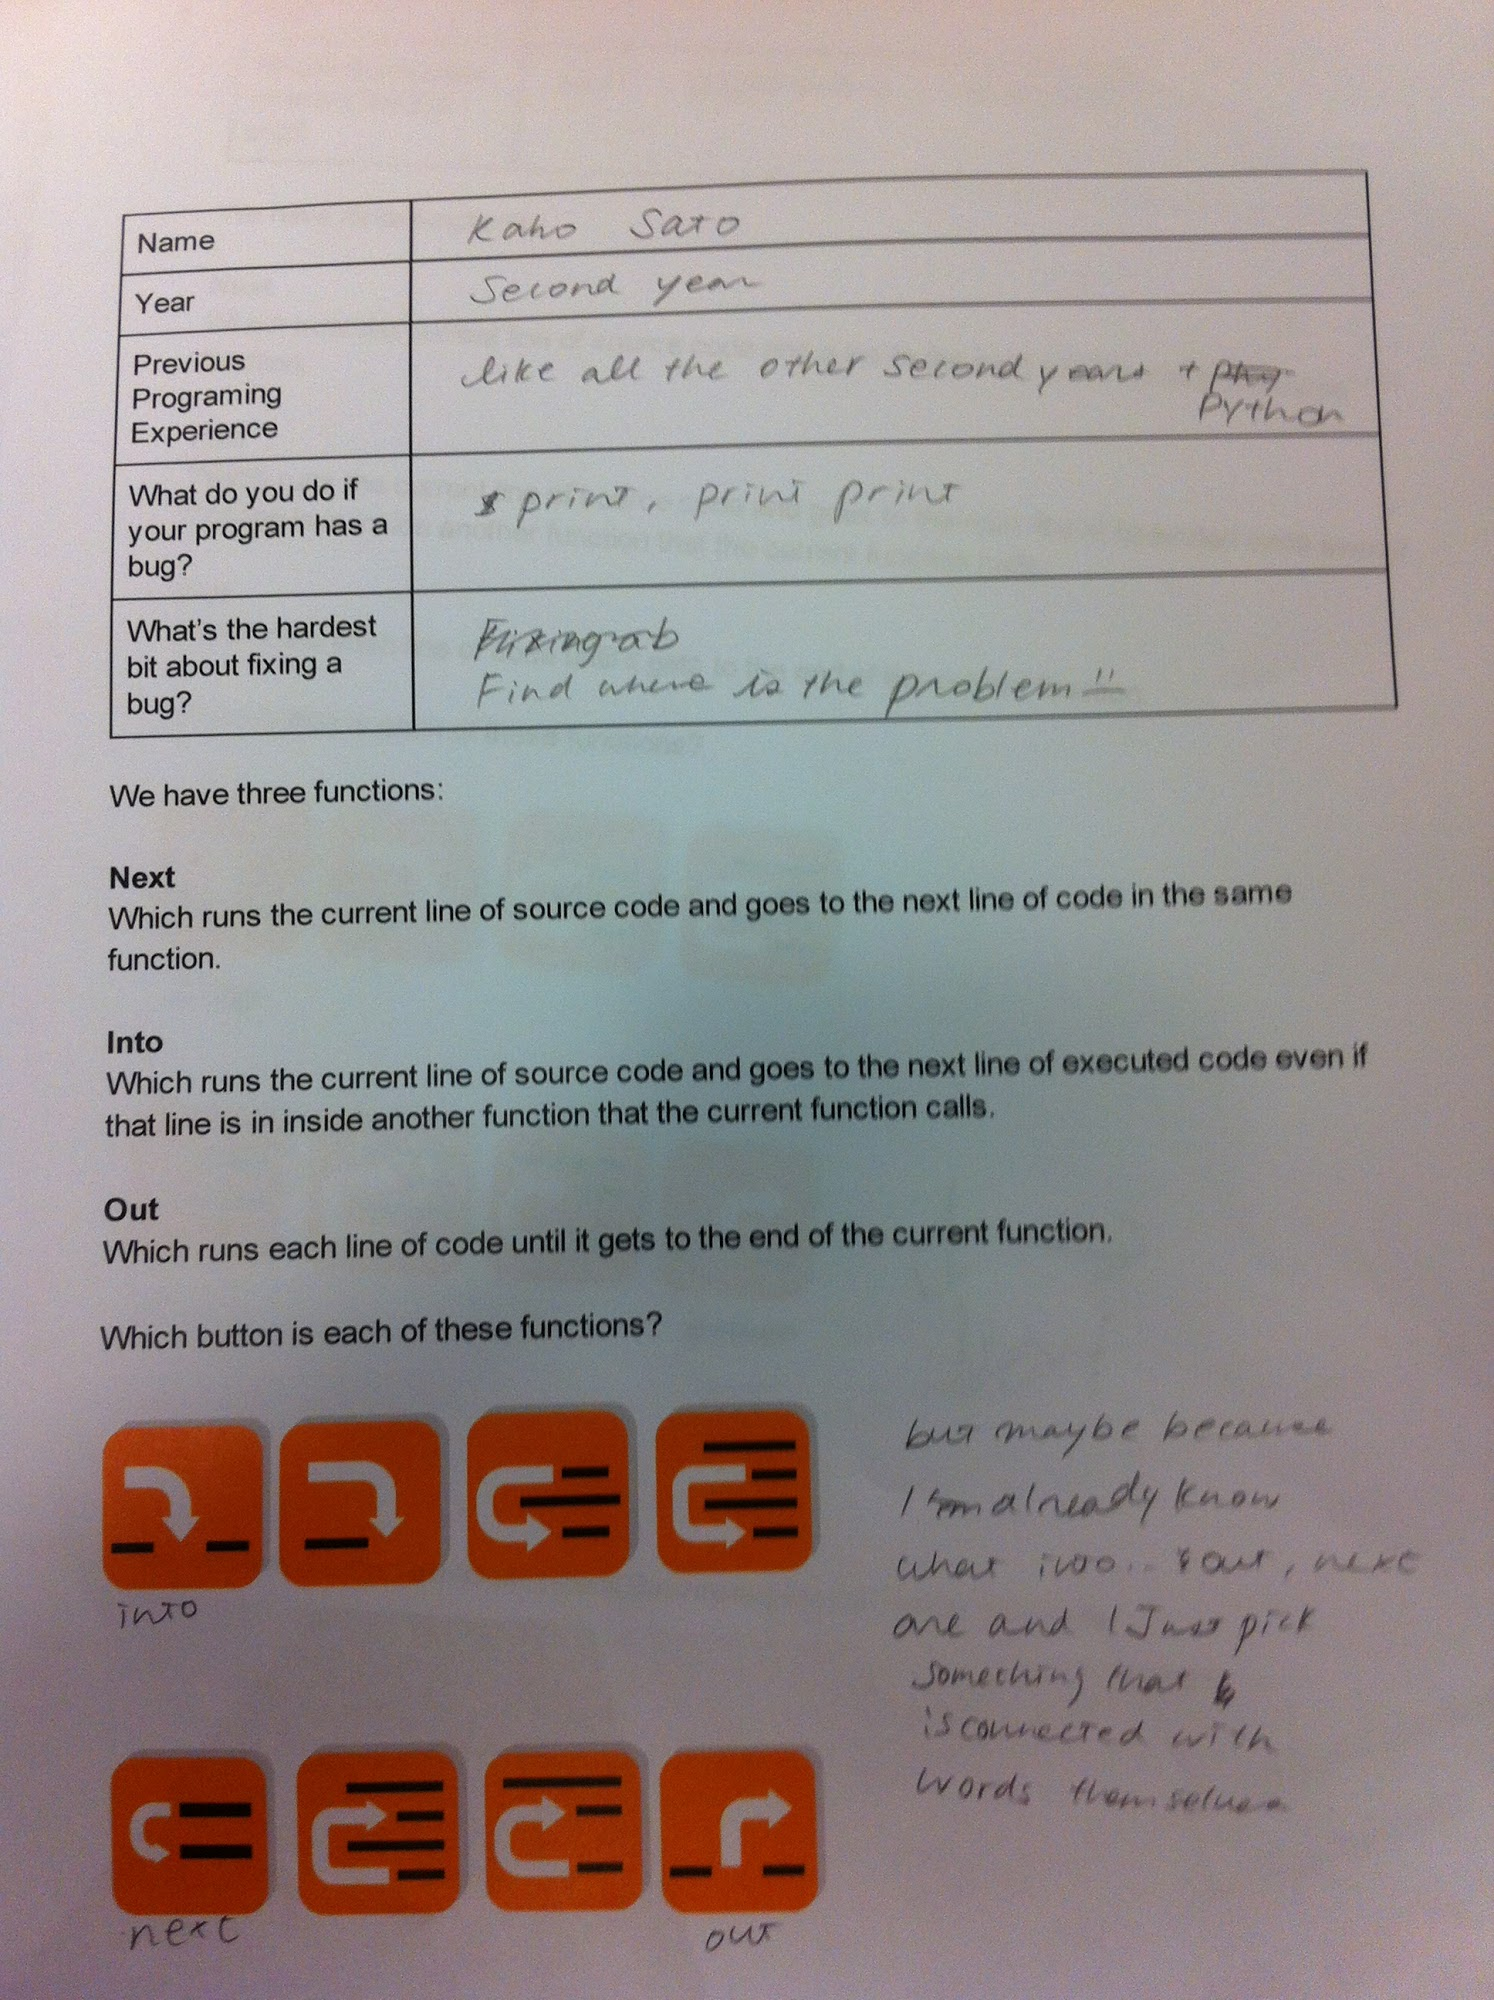
\includegraphics[height=50mm, width=60mm]{questionnair2.jpg}}
\end{figure}

After the general interviews we used a questionnaire to get answers to our most important questions.
Specifically we asked which of the several button designs were better and validated our ad-hoc interview conclusions about the debugger.
We considered using something like Amazon Mechanical Turk to get larger numbers of responses which might have been more statistically significant but it seemed silly when we had hundreds of programmers who were our exact target audience sitting next to us.


\subsection{Performance Testing}
\subsubsection{Time to First Request}
We also used a few other metrics, some custom and some off-the-shelf which could be automatically run over the repository to measure specific aspects of Deeva’s performance.
\begin{figure}[h!]
\centering
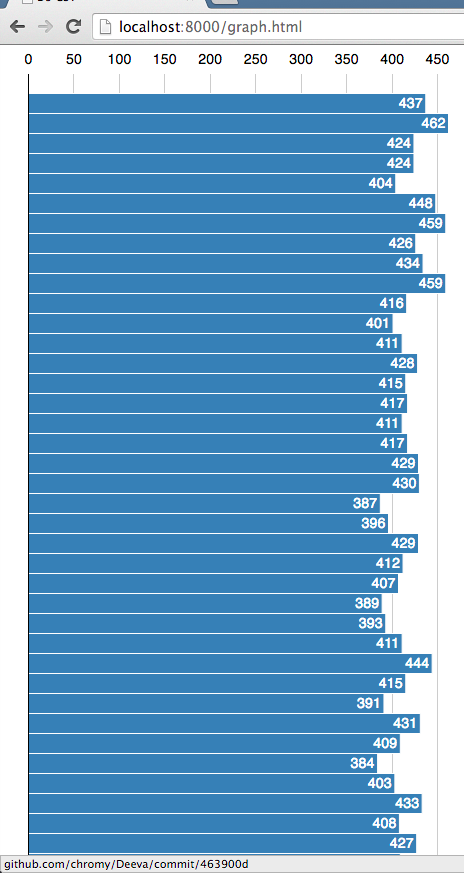
\includegraphics[height=100mm,width=100mm]{timeToFirstRequest.png}
\end{figure}

One of these was the ‘time-to-first-request’.
This is the time it takes Deeva to get from hitting enter on the command line to being able to accept user input.
This is important because tools that are slow to start are painful to use and hence are used less\footnote{ It’s not a direct parallel but if we consider websites, page abandonment approaches 50\% as load time reaches about 10 seconds see: \url{http://blog.kissmetrics.com/loading-time/?wide=1}}.
You can only improve what you measure so we wrote a script that iterates over the git history, starts Deeva and measures the time until it is accepting the first request\footnote{We got the idea for doing this from Gary Bernhardt screencast: \url{https://www.destroyallsoftware.com/screencasts/catalog/time-to-first-request}}.
We can then display the results using a custom D3 graph.

As you can see our app currently takes roughly 450ms to load.
If we see that one commit increased the time-to-first-request, we can click on it and it will take us to the relevant commit on github so we can work out what went wrong.

Happily this has turned out not to be such a big issue on this project as the time-to-first-request quickly stabilised and did not increase dramatically. 

\section{Project Management}
For this project we have three problems which we haven't had (at least in combination) in past university projects: we're not sure what we're building, we want to make sure we deliver the software on time but don't know how long it will take and
we want to make sure the software we write is correct and useful but have no easy way to define `correct' or `useful' in this domain.

Happily Agile Programming has techniques we can use to help solve these problems.
\subsection{Team Member Contributions}
\subsubsection{Kritaphat Sonsri-in}
\subsubsection{Xueqi Chen}
\subsubsection{Alina Draganescu}
\subsubsection{Felix de Souza}
\subsubsection{Hector Dearman}
\subsection{Team Management}

To ensure effective development of the product, weekly supervisor meetings were scheduled.
In these meetings, quality assurance was the main aim, making sure we were on the right track with our development, delivering correct features. 
This avoided unnecessary misunderstandings and extra time spent on creating unneeded features for the product. 

Further to the supervisor meetings, weekly group meetings ensured that all group members are in sync about the progress and direction of the project. 
During these meetings, the information gathered from the supervisor meetings would be recapped and the targets for the upcoming week would be set. 
Thus, tasks could be divided among group members, with everyone knowing what their colleagues are working on in this week, making group and individual efforts significantly more effective.
\begin{figure}[h!]
\centering
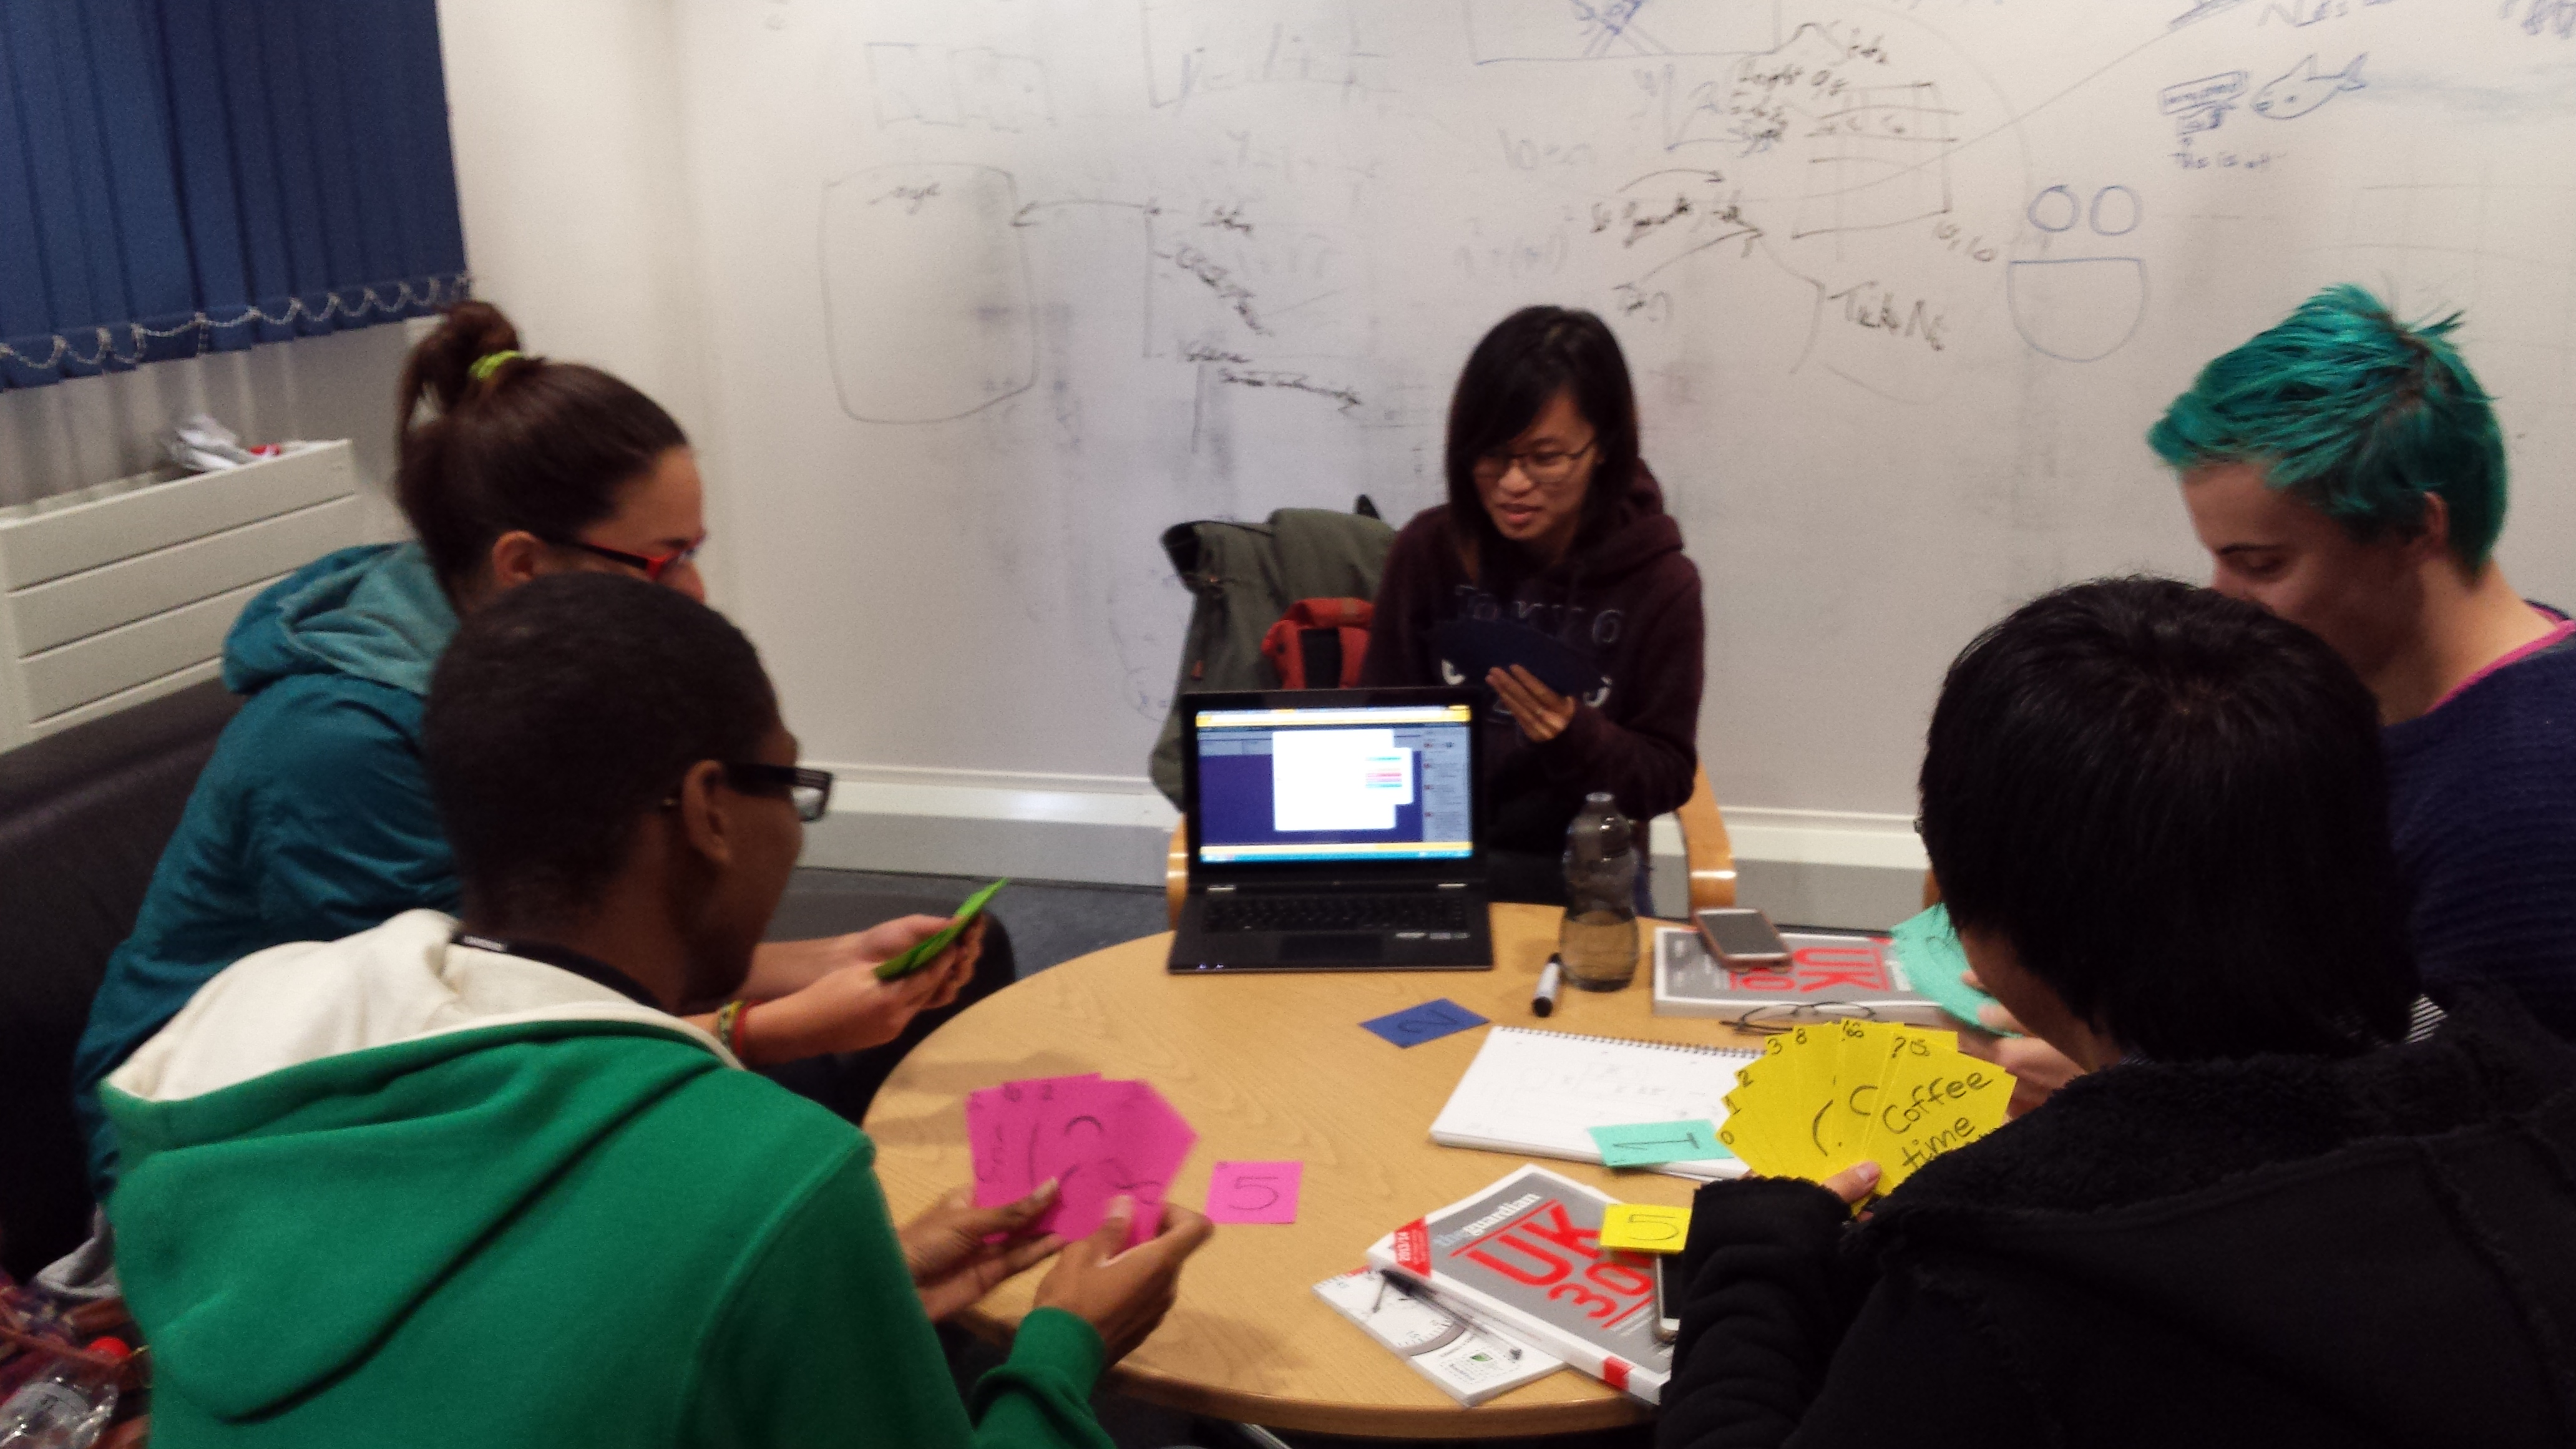
\includegraphics[height=80mm,width=130mm]{estimation.jpg}
\end{figure}

To aid the management of the project on a holistic and timely perspective, several tools were used, which will be outlined in the following section.

\subsection{Tools}
\subsubsection{Trello}
\begin{figure}[h!]
\centering
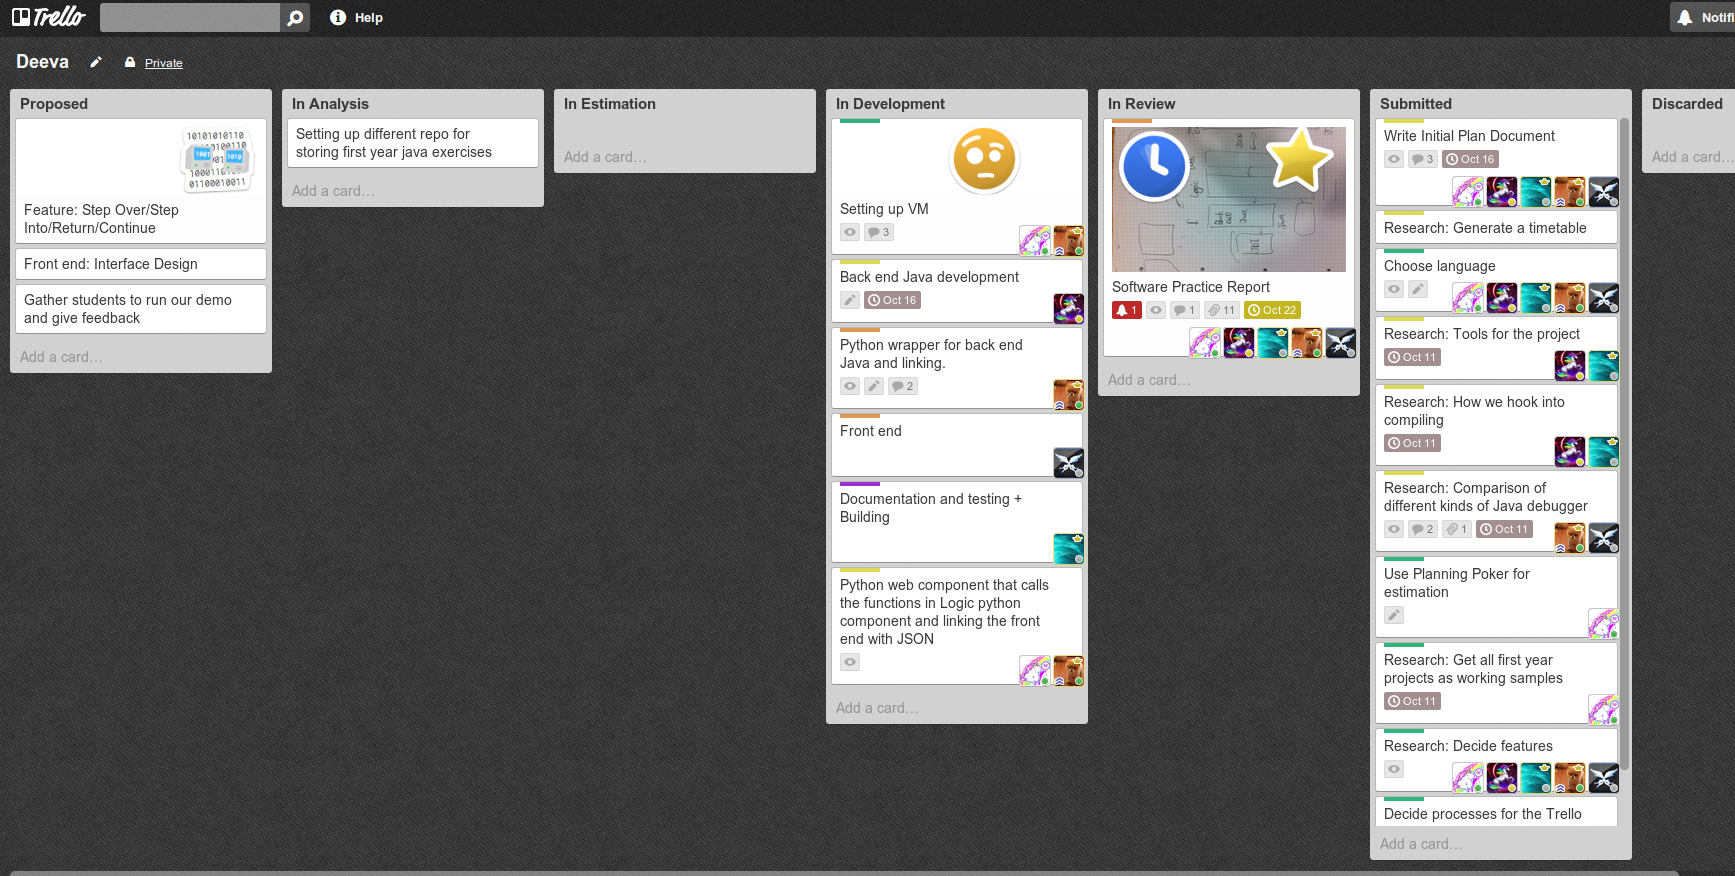
\includegraphics[height=80mm,width=\textwidth]{Trello.png}
\end{figure}

We used Trello as our project management tool and as an Information Radiator\footnote{\url{https://www.atlassian.com/wallboards/information-radiators.jsp}}.
It also allows us to track our progress and average velocity. 
We decided to use Trello as it fulfills most of the key features required for such a tool: it is easy to use and update, relatively flexible and allows for communications between members without too much interruption. 
We decided to use an electronic version as they are a more manageable alternative to physical boards. 
We also found it extremely useful when it came to keeping everyone informed on the general progress and keeping all the information in one compact environment.

A Trello board was created for a better project management process. 
There are several different swimlanes on the board: ``Proposed'', which allows all members to throw in ideas; ``In Analysis'', where people talk about their ideas and have a discussion with group members to see if the story is feasible. 
If it is, the card will be then moved to ``In Estimation'' where we would use Planning Poker to assign the story with a complexity points.
Otherwise, the story will be moved to ``Discarded''.
The reason why we want to keep track of what we have discarded is that we might have thought we would not have time for it, but in reality we may have time at the end.
We might want to move it back and reconsider it. 
After ``In Estimation'', the card will be assigned to group members with a set due date and be moved into ``In Development'' on the Trello board. 
Once the development is complete, the card should be moved into ``In Review''. 
This is when we meet as a group and review our code to improve our style and pattern-usage.

\subsubsection{Planning Poker}
\begin{figure}[h!]
\centering
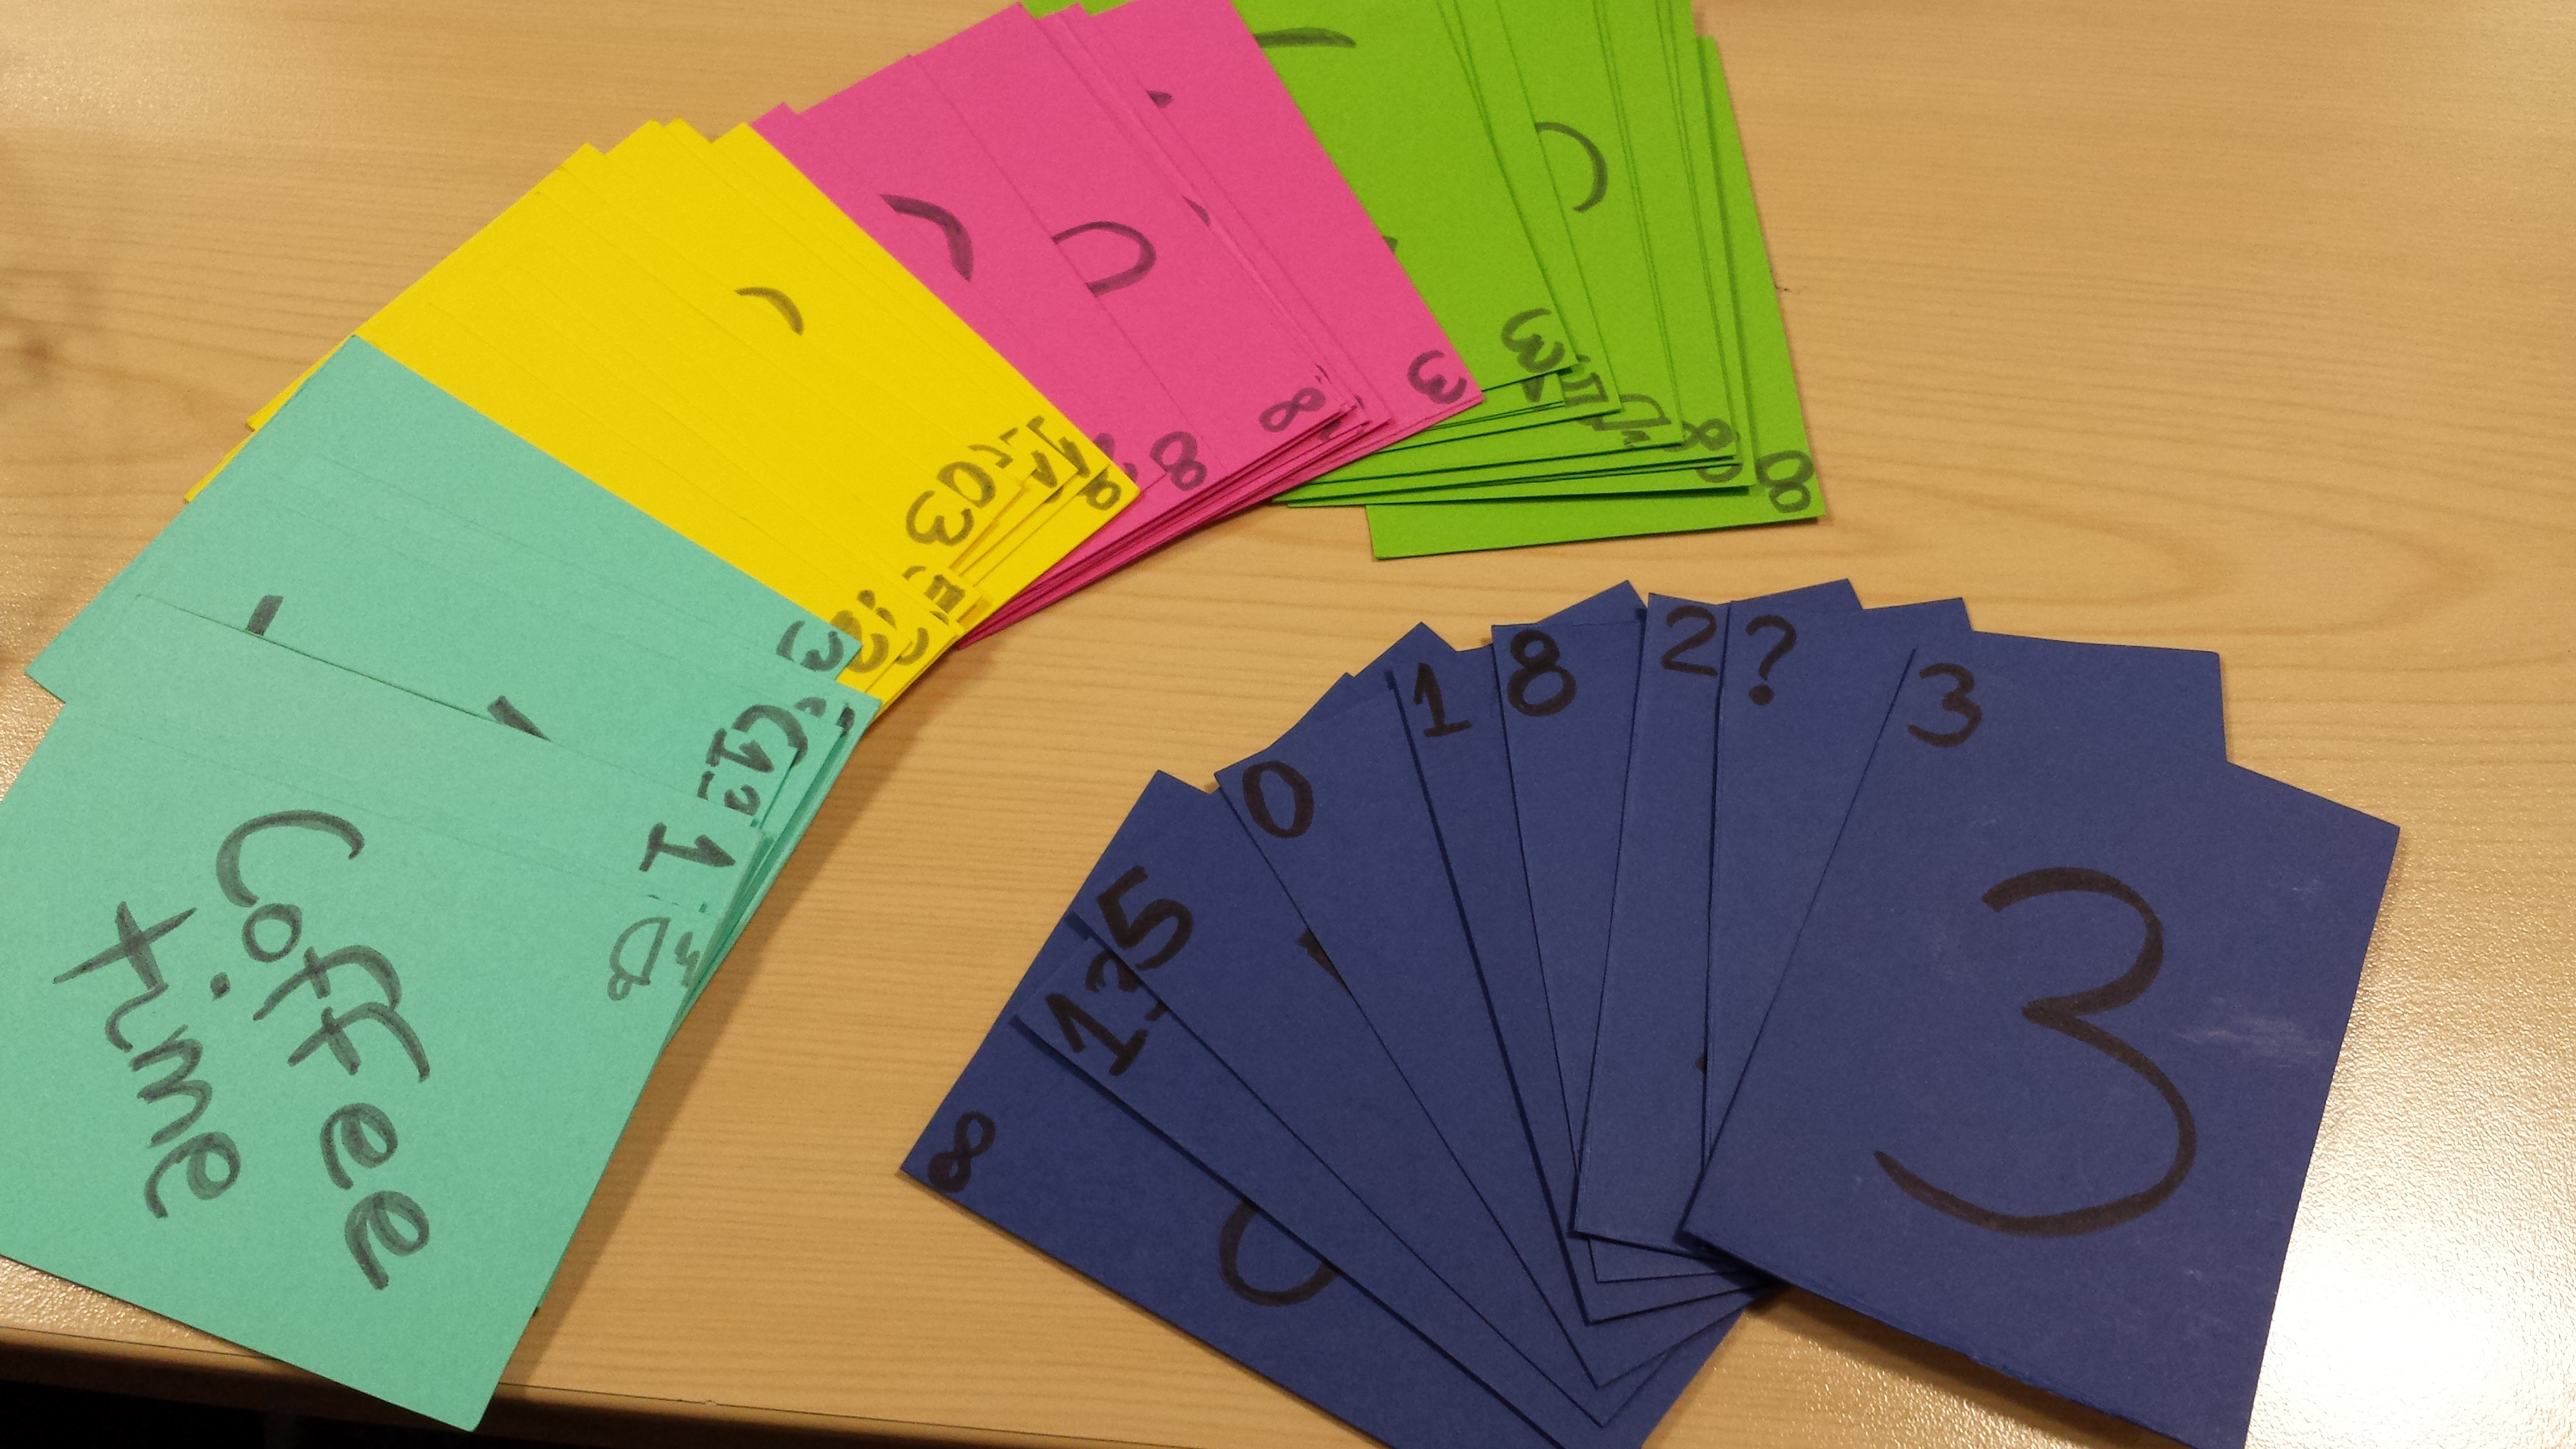
\includegraphics[height=80mm,width=130mm]{planningPokers.jpg}
\end{figure}

We are using Planning Poker in order to estimate stories in each cycle of development. 
This method is known to avoid anchoring and will produce more accurate, less optimistic story point estimations\footnote{\tt{http://en.wikipedia.org/wiki/Planning\_poker\#Planning\_poker\_benefits}}. This technique takes some time to get used to because initially the story point bared little meaning to us.
As we estimated more tasks, the story points became more meaningful hence the poker game proved to be a very efficient method.

For example, it helped determine when people aren't really talking about the same scope for a certain task.
Frequently we have a task like ``Set up the back end." and one person gives a task a 2 while another gives it an 8.
The first person thinks the task title means ``Write some stubs so the middleware can integrate." while the second thinks it means ``Implement the backend up to the minimal specification.". 
So using planing poker has already helped us make sure we're all on the same page.
One of our group members hand-made a set of poker cards just for estimation.
It contains the Fibonacci numbers up to 13 including 0 and infinity - if the task was unfeasible in the time given, as well as ``coffee time'' if we think we needed a break. 

\subsubsection{Facebook Group}
Creating a Facebook group proved very efficient for communicating meeting times and general enquiries that were too conversational for Trello.  

\subsubsection{Google Docs}
We used Google Docs for collaborative editing on reports, plans and meeting summaries in real time.
  
\subsubsection{Github}
Github is a hosted source control which somebody else manages and is easily accessible from anywhere and also plays nicely with the hosted Continuous Integration tool - Travis CI\footnote{\url{http://travis-ci.com/}}.

\subsubsection{Travis CI}
\todo{about Travis here}

\section{Extensions}
\section{Conclusion}

\clearpage
\thispagestyle{empty}
\null\vfill
\begin{center}
\settowidth\longest{``A process cannot be understood by stopping it."}
\parbox{\longest}{%
  \raggedright{%
  ``A process cannot be understood by stopping it." \\
  }   
  \raggedright{\emph{First Law of the Mentat -- Dune}}\par%
}
\end{center}
\addcontentsline{toc}{section}{Quote}
\vfill\vfill
\clearpage

\appendix
\section{Initial Plan}
\label{sec:initialplan}
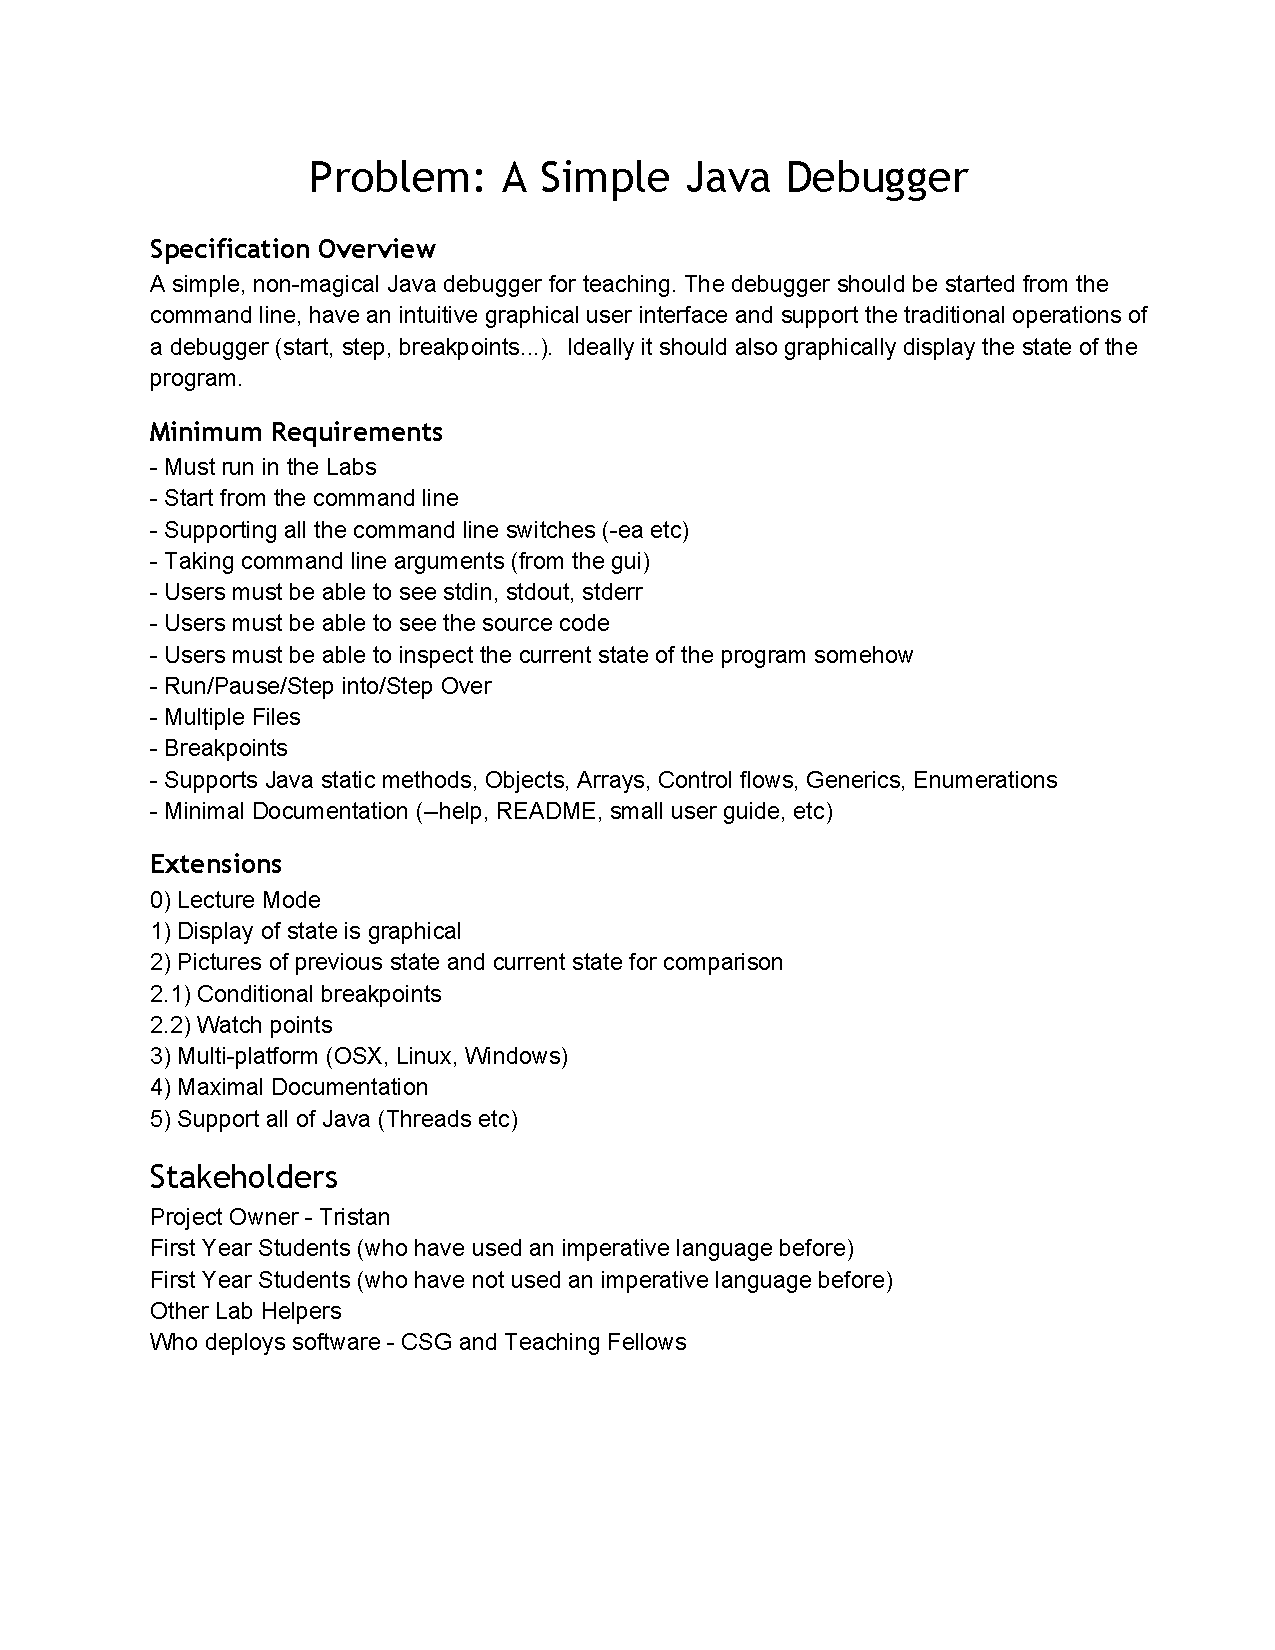
\includepdf[pages={-}, pagecommand={}]{plan.pdf}

\section{Annotated Plan}
\begin{figure}[h!]
\centering
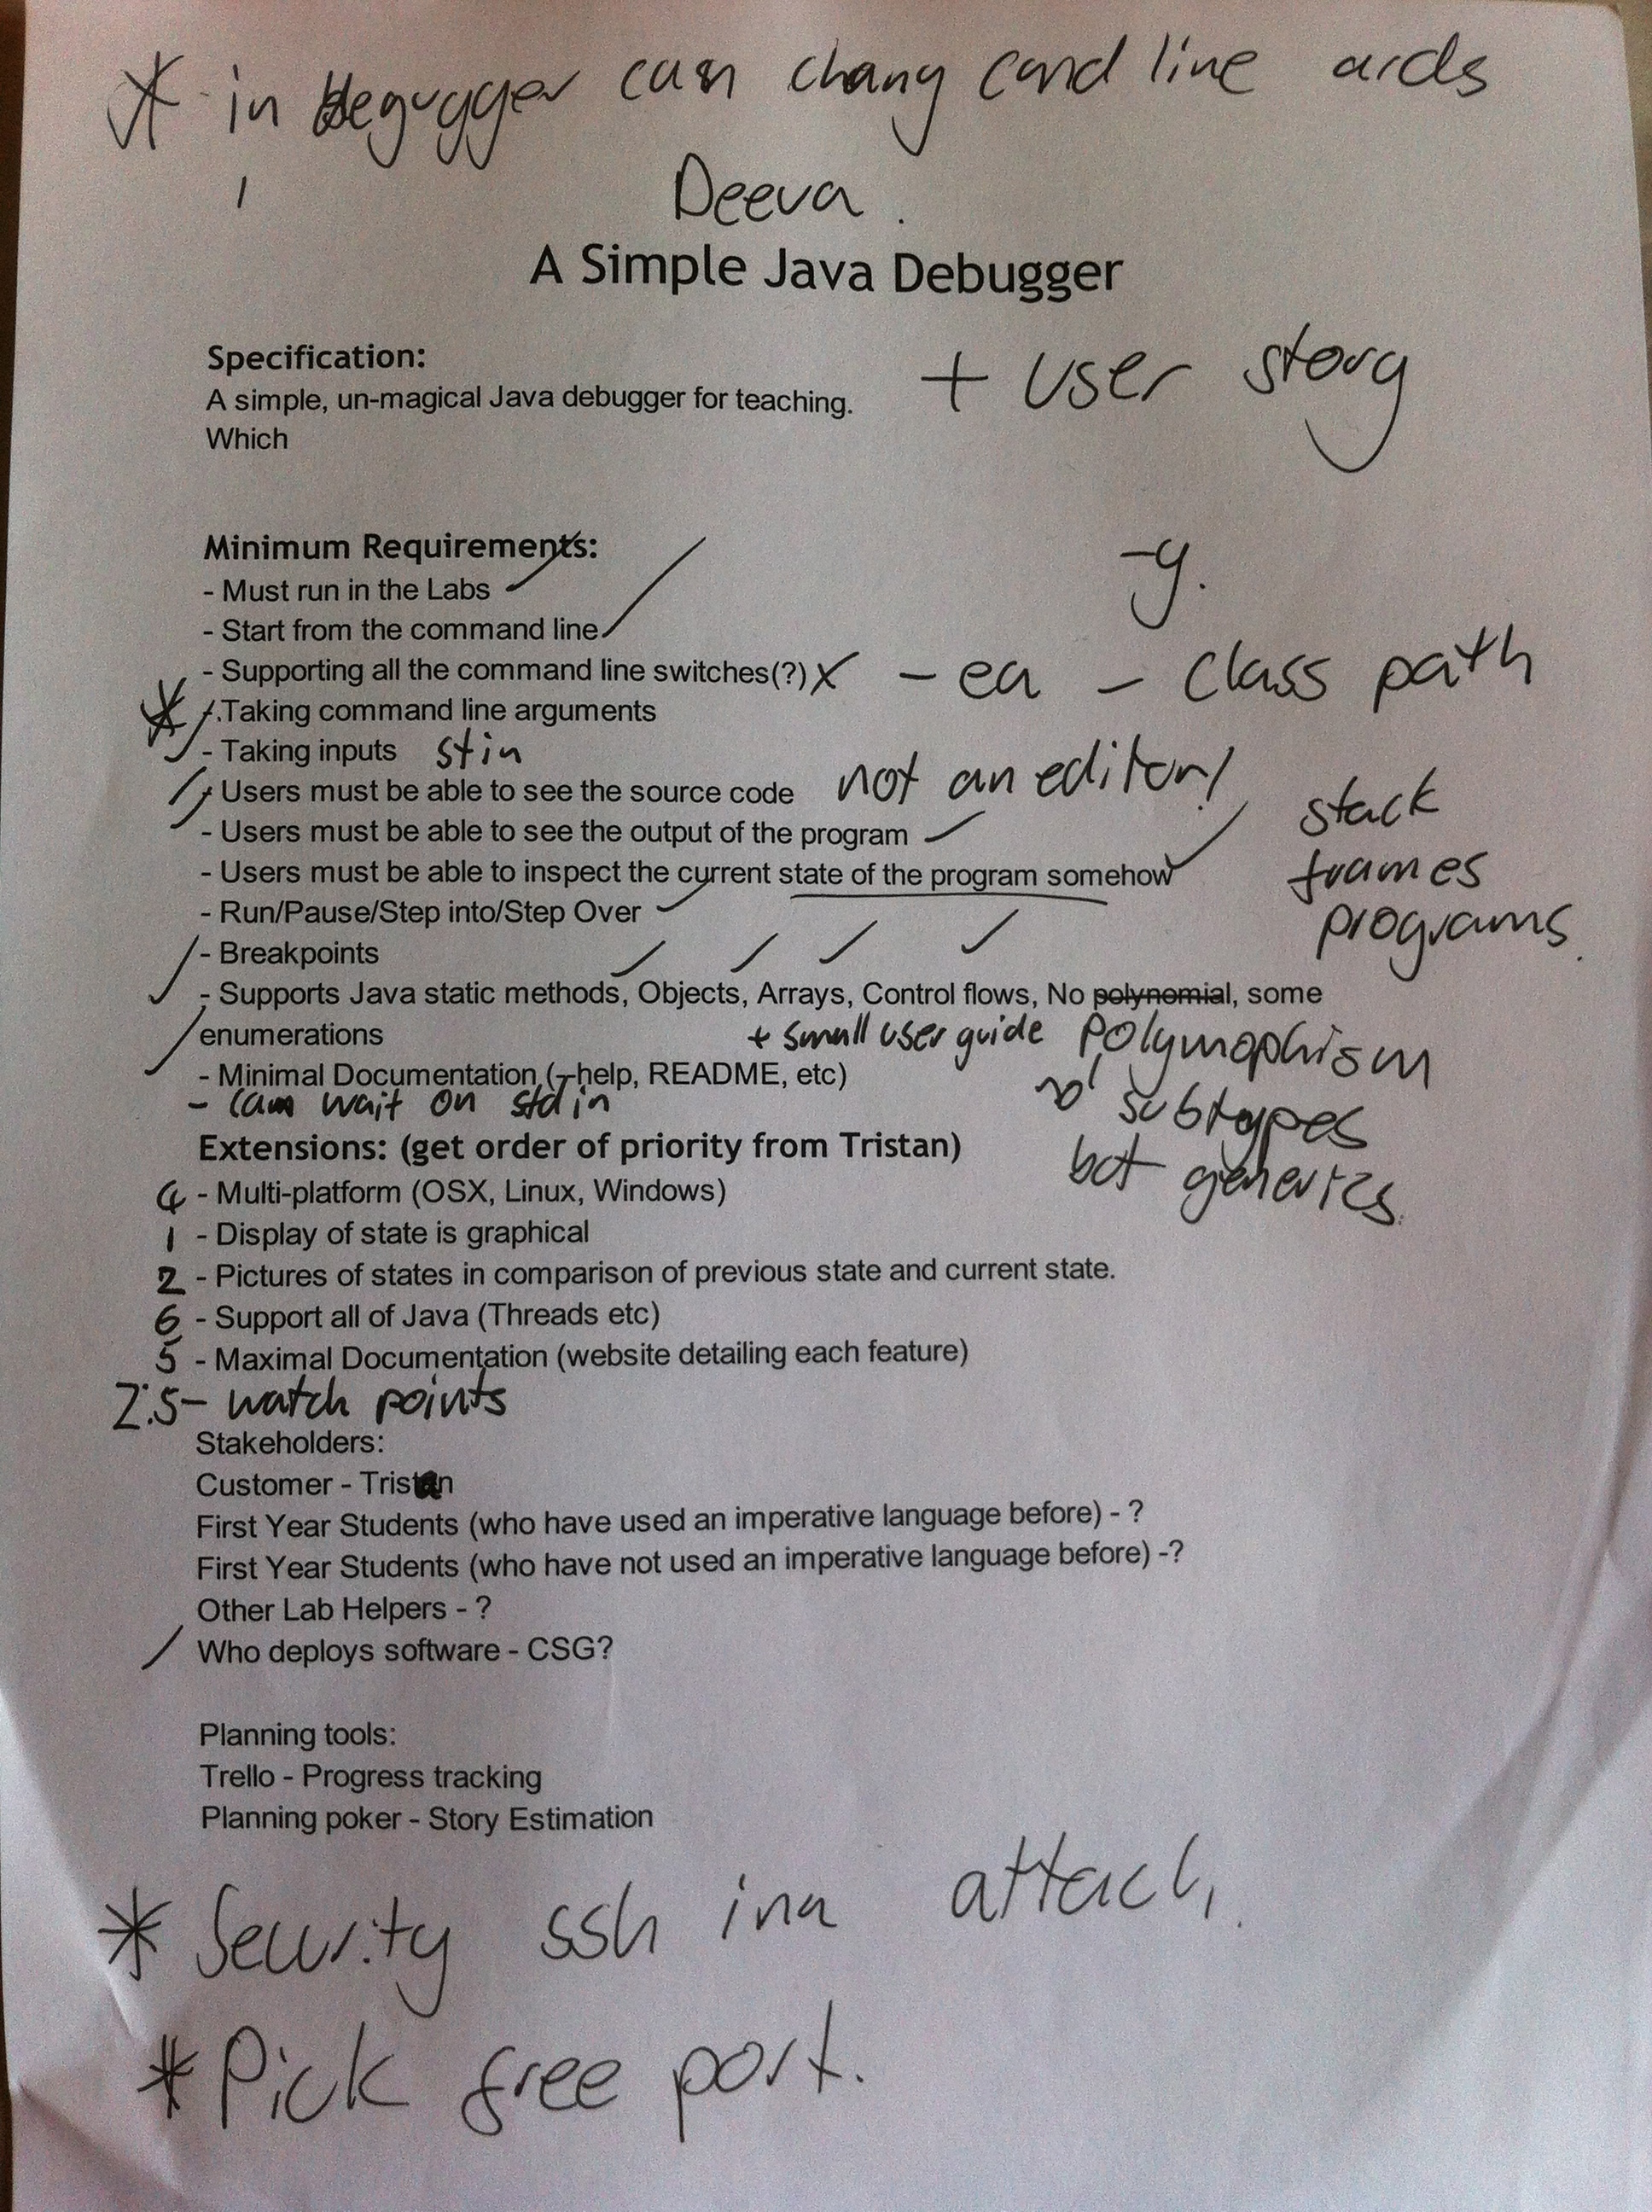
\includegraphics[width=\textwidth]{annotatedreport.jpg}
\caption{An example of notes taken during a meeting with project supervisor.}
\end{figure}

\section{Button Questionnaire}
\label{sec:buttonquestionnaire}
\begin{figure}[h!]
\centering
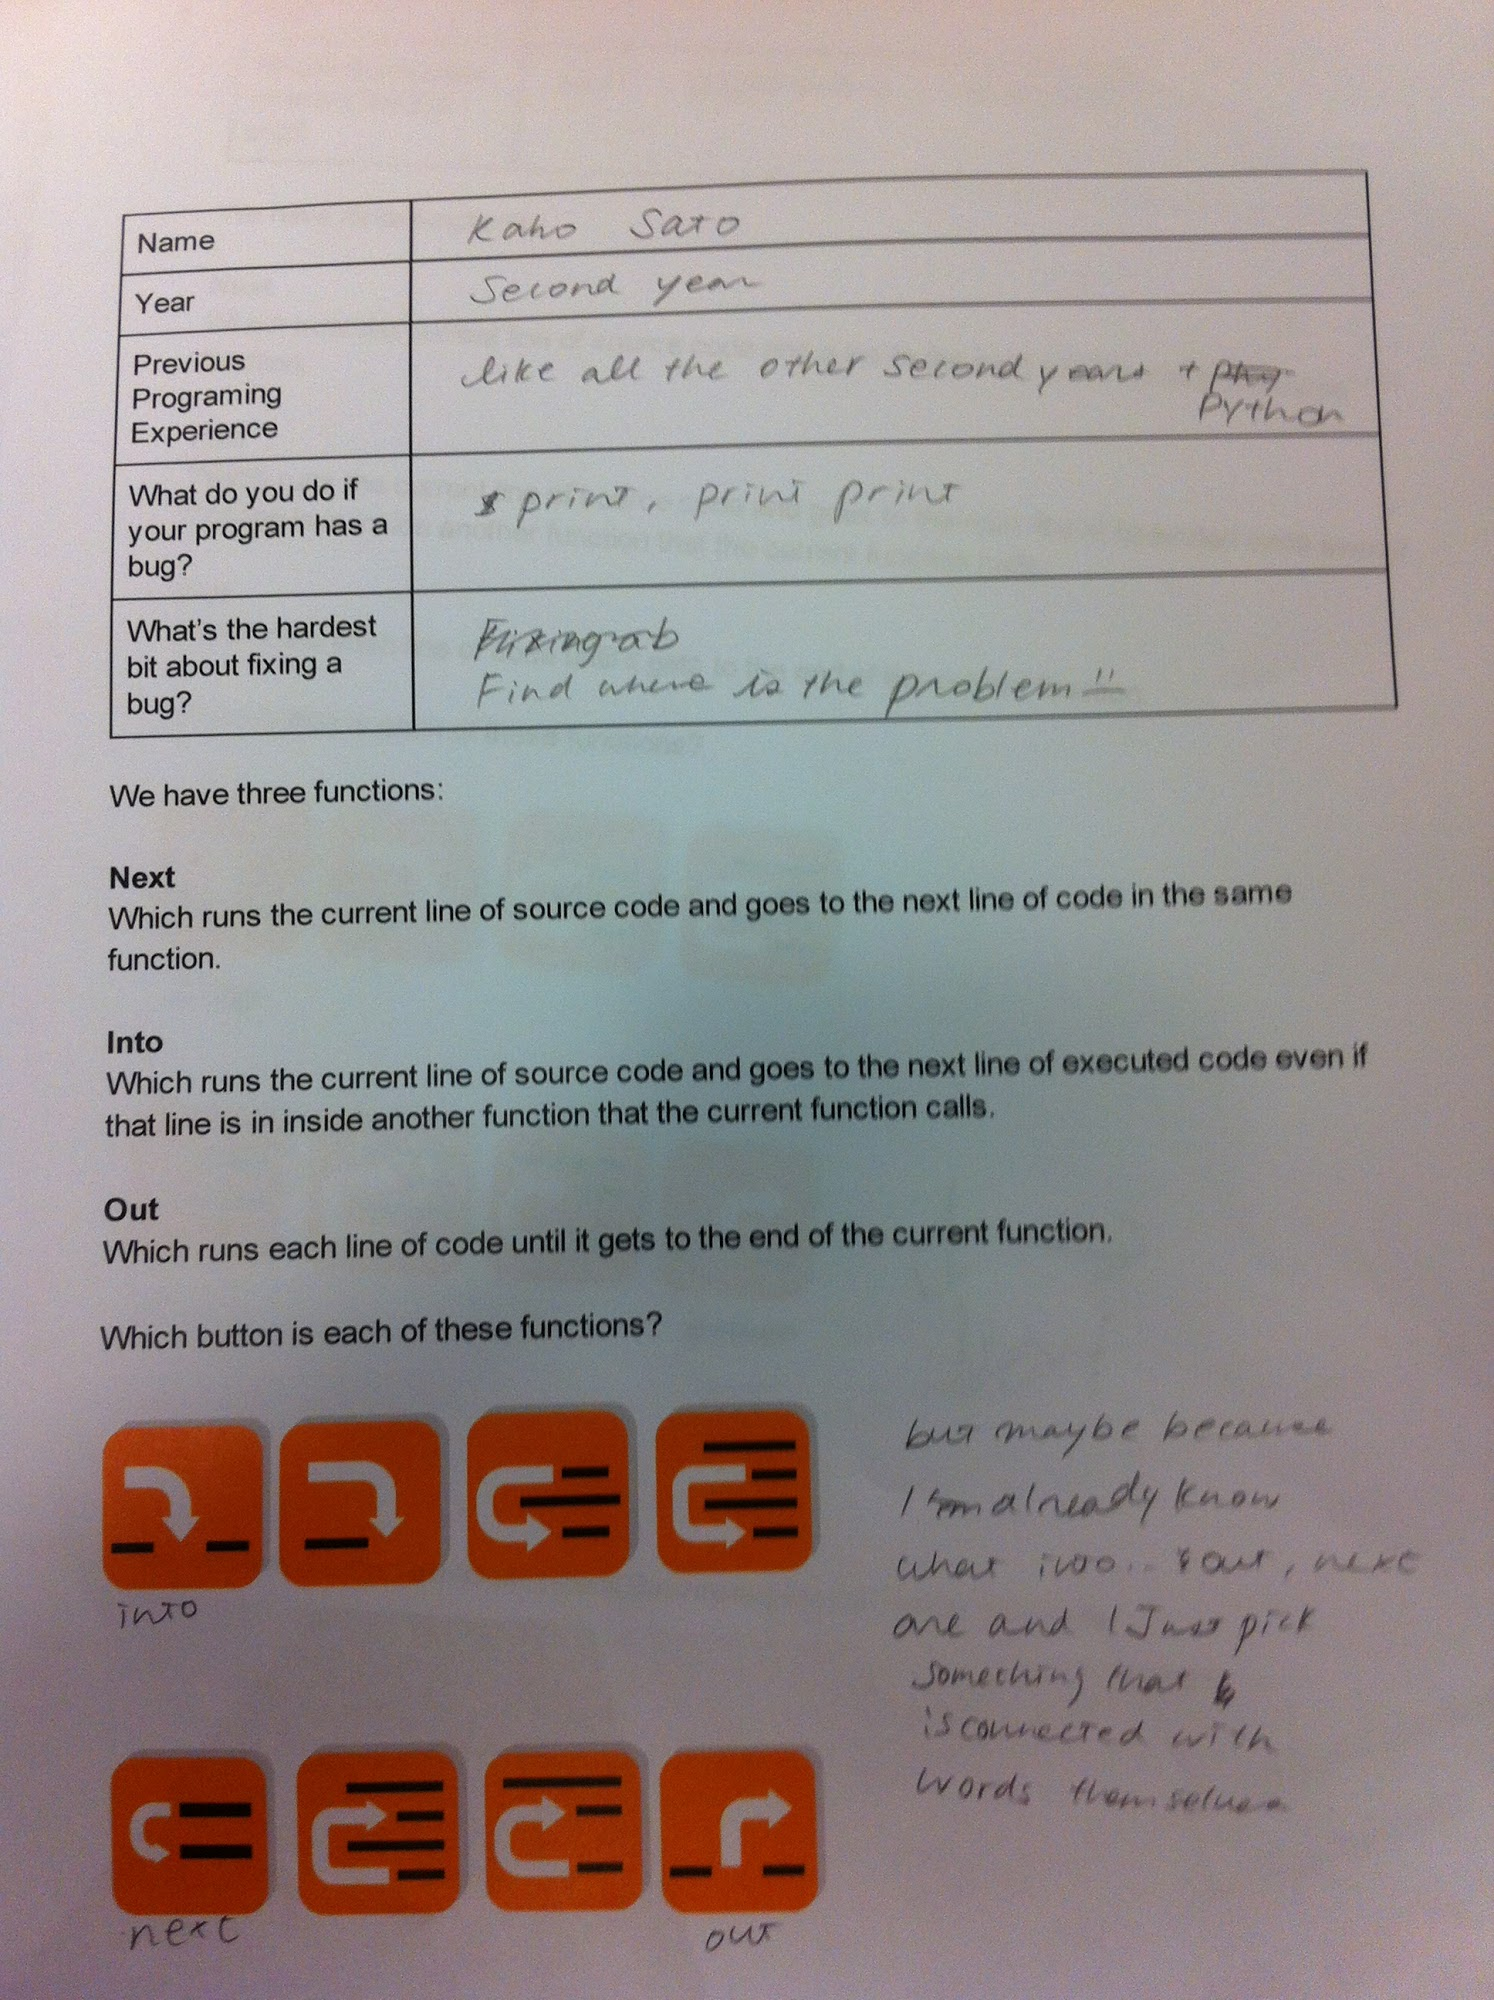
\includegraphics[width=\textwidth]{questionnair2.jpg}
\caption{An example feedback given by a user on our button designs.}
\end{figure}

\section{User Guide}

\begin{thebibliography}{9}

\bibitem{projectproposal}
	Tristan Allwood.
	\emph{Project Proposal: A Java Debugger Suitable for Teaching}.
	\url{https://cate.doc.ic.ac.uk/projects/proposals.cgi?key=2013:1:show-2728}

\bibitem{pythontutor}
	Philip Guo.
	\emph{Python Tutor}.
	\url{http://pythontutor.com/}

\bibitem{saeed09}
	Dehnadi, Saeed, Richard Bornat, and Ray Adams. 
	\emph{Meta-analysis of the effect of consistency on success in early learning of programming.}
	PPIG, 2009.
\end{thebibliography}

\end{document}
